% This is the Reed College LaTeX thesis template. Most of the work
% for the document class was done by Sam Noble (SN), as well as this
% template. Later comments etc. by Ben Salzberg (BTS). Additional
% restructuring and APA support by Jess Youngberg (JY).
% Your comments and suggestions are more than welcome; please email
% them to cus@reed.edu
%
% See http://web.reed.edu/cis/help/latex.html for help. There are a
% great bunch of help pages there, with notes on
% getting started, bibtex, etc. Go there and read it if you're not
% already familiar with LaTeX.
%
% Any line that starts with a percent symbol is a comment.
% They won't show up in the document, and are useful for notes
% to yourself and explaining commands.
% Commenting also removes a line from the document;
% very handy for troubleshooting problems. -BTS

% As far as I know, this follows the requirements laid out in
% the 2002-2003 Senior Handbook. Ask a librarian to check the
% document before binding. -SN

%%
%% Preamble
%%
% \documentclass{<something>} must begin each LaTeX document
\documentclass[12pt,twoside]{reedthesis}
% Packages are extensions to the basic LaTeX functions. Whatever you
% want to typeset, there is probably a package out there for it.
% Chemistry (chemtex), screenplays, you name it.
% Check out CTAN to see: http://www.ctan.org/
%%
\usepackage{graphicx,latexsym}
\usepackage{amsmath}
\usepackage{amssymb,amsthm}
\usepackage{longtable,booktabs,setspace}
\usepackage{chemarr} %% Useful for one reaction arrow, useless if you're not a chem major
\usepackage[hyphens]{url}
% Added by CII
\usepackage{hyperref}
\usepackage{lmodern}
\usepackage{float}
\floatplacement{figure}{H}
% End of CII addition
\usepackage{rotating}

% Next line commented out by CII
%%% \usepackage{natbib}
% Comment out the natbib line above and uncomment the following two lines to use the new
% biblatex-chicago style, for Chicago A. Also make some changes at the end where the
% bibliography is included.
%\usepackage{biblatex-chicago}
%\bibliography{thesis}


% Added by CII (Thanks, Hadley!)
% Use ref for internal links
\renewcommand{\hyperref}[2][???]{\autoref{#1}}
\def\chapterautorefname{Chapter}
\def\sectionautorefname{Section}
\def\subsectionautorefname{Subsection}
% End of CII addition

% Added by CII
\usepackage{caption}
\captionsetup{width=5in}
% End of CII addition

% \usepackage{times} % other fonts are available like times, bookman, charter, palatino


% To pass between YAML and LaTeX the dollar signs are added by CII
\title{Local Dependence in Exponential Random Network Models}
\author{Nicholas Solomon}
% The month and year that you submit your FINAL draft TO THE LIBRARY (May or December)
\date{May 2017}
\division{Mathematics and Natural Sciences}
\advisor{Albyn Jones}
%If you have two advisors for some reason, you can use the following
% Uncommented out by CII
% End of CII addition

%%% Remember to use the correct department!
\department{Mathematics - Statistics}
% if you're writing a thesis in an interdisciplinary major,
% uncomment the line below and change the text as appropriate.
% check the Senior Handbook if unsure.
%\thedivisionof{The Established Interdisciplinary Committee for}
% if you want the approval page to say "Approved for the Committee",
% uncomment the next line
%\approvedforthe{Committee}

% Added by CII
%%% Copied from knitr
%% maxwidth is the original width if it's less than linewidth
%% otherwise use linewidth (to make sure the graphics do not exceed the margin)
\makeatletter
\def\maxwidth{ %
  \ifdim\Gin@nat@width>\linewidth
    \linewidth
  \else
    \Gin@nat@width
  \fi
}
\makeatother

\renewcommand{\contentsname}{Table of Contents}
% End of CII addition

\setlength{\parskip}{0pt}

% Added by CII

\providecommand{\tightlist}{%
  \setlength{\itemsep}{0pt}\setlength{\parskip}{0pt}}

\Acknowledgements{
First and foremost, this thesis is due to all of the professors at Reed
who have taught, encouraged, and guided me during my time here.
Obviously, my adviser, Albyn Jones, had the largest impact on this
document. Thank you for putting up with my silly mistakes and keeping me
on track. I also have to thank you for teaching me statistics in the
first place. Math 392 is the reason I am where I am today.

I also have to thank Andrew Bray, Chester Ismay, and Jim Fix for their
contributions to this project. On more than one occasion, each of them
took the time out of their busy schedules to listen to me complain about
my thesis. Without them, I would not have been able to get as far as I
did.

Finally, I owe a debt to Jerry Shurman, who, as my sophomore year
adviser, insisted I have some useful skill upon graduating from Reed.
Without him, I never would have taken a statistics class and this thesis
would be about complex analysis.

Equally as important as my professors, this project is due to my family.
My parents have provided unwavering love and support during my time
here. They also paid my tuition.

Last but not least, I want to thank all the friends I made here. You
know who you are, and if you think this is meant for you, then it is.
}

\Dedication{

}

\Preface{

}

\Abstract{
Graph representations are used across disciplines for the analysis and
visualization of relational data. Exponential random graph models allow
for a general method of modelling the underlying stochastic process that
has generated the observed data conditional on observer attributes of
the vertices, or nodes. Recent developments in ERGMs have introduced the
notions of local dependence and the exponential random network model, or
ERNM. Local dependence enforces the assumption of independence between
edges that connect nodes that are, in some sense, ``far apart.'' This is
formalized by the introduction of a neighborhood structure on the graph:
a partition of the vertices with the property that edges between two
neighborhoods are stochastically independent of all other edge
variables. This independence allows for the proof of a desirable
consistency condition and a central limit theorem for statistics of the
graph. The random network model allows for the joint modelling of both
the graph and random attributes of the vertices. This has useful
applications in network analysis, as it allows researchers to make
inferences about how graphical features affect vertices and vice versa.
This thesis combines these two developments to show that ERNMs with the
local dependence property have the same useful consistency property and
that a similar central limit theorem also holds.
}

	\usepackage{tikz}
	\usetikzlibrary{shapes}
	\usetikzlibrary{arrows.meta}
% End of CII addition
%%
%% End Preamble
%%
%

\usepackage{amsthm}
\newtheorem{theorem}{Theorem}[chapter]
\newtheorem{lemma}{Lemma}[chapter]
\theoremstyle{definition}
\newtheorem{definition}{Definition}[chapter]
\newtheorem{corollary}{Corollary}[chapter]
\newtheorem{proposition}{Proposition}[chapter]
\theoremstyle{definition}
\newtheorem{example}{Example}[chapter]
\theoremstyle{remark}
\newtheorem*{remark}{Remark}
\let\BeginKnitrBlock\begin \let\EndKnitrBlock\end
\begin{document}

% Everything below added by CII
  \maketitle

\frontmatter % this stuff will be roman-numbered
\pagestyle{empty} % this removes page numbers from the frontmatter
  \begin{acknowledgements}
    First and foremost, this thesis is due to all of the professors at Reed
    who have taught, encouraged, and guided me during my time here.
    Obviously, my adviser, Albyn Jones, had the largest impact on this
    document. Thank you for putting up with my silly mistakes and keeping me
    on track. I also have to thank you for teaching me statistics in the
    first place. Math 392 is the reason I am where I am today.
    
    I also have to thank Andrew Bray, Chester Ismay, and Jim Fix for their
    contributions to this project. On more than one occasion, each of them
    took the time out of their busy schedules to listen to me complain about
    my thesis. Without them, I would not have been able to get as far as I
    did.
    
    Finally, I owe a debt to Jerry Shurman, who, as my sophomore year
    adviser, insisted I have some useful skill upon graduating from Reed.
    Without him, I never would have taken a statistics class and this thesis
    would be about complex analysis.
    
    Equally as important as my professors, this project is due to my family.
    My parents have provided unwavering love and support during my time
    here. They also paid my tuition.
    
    Last but not least, I want to thank all the friends I made here. You
    know who you are, and if you think this is meant for you, then it is.
  \end{acknowledgements}

  \hypersetup{linkcolor=black}
  \setcounter{tocdepth}{1}
  \tableofcontents

  \listoftables

  \listoffigures
  \begin{abstract}
    Graph representations are used across disciplines for the analysis and
    visualization of relational data. Exponential random graph models allow
    for a general method of modelling the underlying stochastic process that
    has generated the observed data conditional on observer attributes of
    the vertices, or nodes. Recent developments in ERGMs have introduced the
    notions of local dependence and the exponential random network model, or
    ERNM. Local dependence enforces the assumption of independence between
    edges that connect nodes that are, in some sense, ``far apart.'' This is
    formalized by the introduction of a neighborhood structure on the graph:
    a partition of the vertices with the property that edges between two
    neighborhoods are stochastically independent of all other edge
    variables. This independence allows for the proof of a desirable
    consistency condition and a central limit theorem for statistics of the
    graph. The random network model allows for the joint modelling of both
    the graph and random attributes of the vertices. This has useful
    applications in network analysis, as it allows researchers to make
    inferences about how graphical features affect vertices and vice versa.
    This thesis combines these two developments to show that ERNMs with the
    local dependence property have the same useful consistency property and
    that a similar central limit theorem also holds.
  \end{abstract}

\mainmatter % here the regular arabic numbering starts
\pagestyle{fancyplain} % turns page numbering back on

\chapter{Introduction}\label{introduction}

\section{Random graphs}\label{random-graphs}
\begin{figure}

{\centering 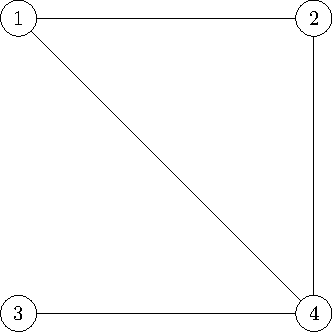
\includegraphics{figure/small_net} 

}

\caption{An undirected graph on four vertices.}\label{fig:graph}
\end{figure}
The mathematical object we call a graph is a set of vertices and edges,
so for a graph \(G\), we write \(G = (V, E)\) where \(V\) is the set of
vertices and \(E\) are ordered or unordered pairs \((i, j)\) for
\(i, j \in V\). These objects can be represented visually by pictures
like Figure \ref{fig:graph}. If the pairs in \(E\) are ordered, then we
say that \(G\) is directed (or sometimes that \(G\) is a digraph),
otherwise we say that \(G\) is undirected. The example in Figure
\ref{fig:graph} is undirected; when drawing directed graph, we can
indicate the direction of the the edge \((i, j)\) by drawing an arrow
from node \(i\) to node \(j\), as in Figure \ref{fig:digraph}. If we
only consider the presence or absence of an edge between vertices, then
we say that the graph \(G\) is unweighted. In a weighted graph, each
edge is assigned a numeric value, called the weight. The case of an
unweighted graph is equivalent a weighted graph where each edge weight
\(w_{ij} \in \{0,1\} \).
\begin{figure}

{\centering 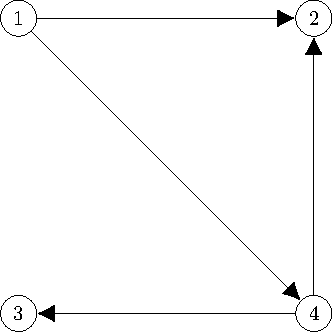
\includegraphics{figure/small_net_di} 

}

\caption{A directed graph on four vertices}\label{fig:digraph}
\end{figure}
Generally, the most convenient way to represent a graph is as an
adjacency matrix. For a graph with \(n\) vertices, the adjacency matrix
is the \(n \times n\) matrix with the weight of edge \((i,j)\) in the
\(i, j\) position. Note that if a graph \(G\) is undirected, then its
adjacency matrix is symmetric and if \(G\) is an unweighted graph, then
all its entries are either \(1\) or \(0\). For example, the graph in
Figure \ref{fig:graph} has adjacency matrix
\begin{equation}
\begin{bmatrix}
0 & 1 & 0 & 1 \\
1 & 0 & 0 & 1 \\
0 & 0 & 0 & 1 \\
1 & 1 & 1 & 0
\end{bmatrix}.
\label{eq:adj-mat}
\end{equation}
Here, we have adopted the convention that vertices do not have an edge
with themselves, so the diagonal elements of this matrix are all zero.
Sometimes we will also represent a graph as an edge list, which is
simply the set of pairs in \(E\) with their weights.

If we assume that a graph \(G\) is generated by some kind of stochastic
process, then we consider the whole graph as a random variable. This is
equivalent to considering the random matrix \(Y\), where \(Y\) is the
adjacency matrix of \(G\). We can consider the \(n^2\) random variables
\(Y_{ij}\) for \(i, j \in \{1, \dots, n\}\), taking values in the set of
possible weights for the random graph in consideration. For example, if
\(G\) is an undirected binary random graph, then this can be simplified
to the \(n^2/2 - n\) Bernoulli random variables \(Y_{(i, j)}\) for
\(1 \leq i \leq j \leq n\). By breaking the random graph into these
simpler parts, we can begin to apply familiar statistical ideas to these
complex objects.

\section{Network modeling}\label{network-modeling}

Graphs are a convenient way to represent relational data, or data that
contain information about a relationship between actors. This brings us
to the area of network analysis, where random graphs are used to model
many different kinds of relationships. For example, in sociology,
networks are commonly used to model relationships among people, like
marriages within a group of people. Political scientists use random
graphs to represent things like the network of trade agreements between
nations. Finally, in epidemiology, random networks can model an
underlying contact network, say of people who shake hands or otherwise
come into contact in a way that could spread a disease, over which a
transmissible infection spreads. This allows the researcher to estimate
how the medical features of the disease and the sociological features of
the population interact to promote or inhibit the spread of disease. As
an example of this, see Groendyke, Welch, \& Hunter
(\protect\hyperlink{ref-Groendyke2012}{2012}), where, among other
things, they examine if closing schools would have had an effect on the
spread of an 1861 measles outbreak.

To formalize these notions, we begin with a random graph \(Y\) on \(n\)
vertices (called nodes in the field of network analysis) considered as a
random matrix with sample space \(\mathcal{Y},\) where \(\mathcal{Y}\)
is the set of all possible graphs on \(n\) vertices. There may be some
restrictions on \(\mathcal{Y}\), depending on the application being
considered. Usually, we prohibit edges that connect a vertex to itself
by forcing the diagonal entries of \(Y\) to be \(0\), as in
\eqref{eq:adj-mat}. However, specific contexts may require nonobvious
constraints put in place by the researcher; for example, when using a
network to model the romantic relationships within a group of people,
the researcher must exclude networks with ties between nodes that do not
have the appropriate gender, depending on the respective preferences of
each pair of nodes.

This thesis explores two classes of network models: the exponential
random graph model (ERGM) and the exponential random network model
(ERNM). These models are quite similar in that they both model the
structural features of the network, such as node degree and triangle
formation, as a function of nodal covariates, say age or gender.
However, the ERNM also models the effect of network features on the
nodes. For example, Fellows \& Handcock
(\protect\hyperlink{ref-Fellows2012}{2012}) show that teens with friends
who smoke or drink are more likely to smoke or drink themselves.

The notion of local dependence was introduced by Schweinberger \&
Handcock (\protect\hyperlink{ref-Schweinberger2015}{2015}) in the
context of ERGMs. Here we extend this idea to ERNMs and provide new
proofs of their two main theorems in this context. The first theorem
shows that the stochastic process of sampling smaller subnetworks from a
large network satisfies a desirable consistency condition. This means
that as we sample larger and larger subnetworks, the model parameter
estimates become better and better approximations of the true parameter
values. Shalizi \& Rinaldo (\protect\hyperlink{ref-Shalizi2013}{2013})
showed that this is not the case for most ERGMs. The second theorem
shows that certain types of statistics of locally dependent random
networks have an asymptotically normal distribution, which is also
desirable from the point of view of making inferences based on these
models.

\chapter{Exponential random graph
models}\label{exponential-random-graph-models}

The first model of interest to this thesis is the exponential random
graph model (ERGM), introduced by S. Wasserman \& Pattison
(\protect\hyperlink{ref-Wasserman1996}{1996}). Broadly, given a network,
this model allows us to specify structural features that are of interest
and test in a principled way if there are more of those kinds of
features present than would be expected if the network were formed by
chance. This allows the researcher to draw conclusions about the latent
process that generated the network.

This model can be expressed by the equation
\begin{equation}
  P(Y = y | \theta) = \frac{e^{\theta \cdot g(y)}}{C(\theta, \mathcal{Y})}
  \label{eq:ergm},
\end{equation}
where \(g(y)\) is a vector of statistics that depend on the network
\(y\) and \(\theta\) is a vector of parameters. The function
\(C(\theta, \mathcal{Y})\) is a normalizing constant. We may easily
extend the model to include nodal covariates (like demographic
information) by introducing the fixed \(n \times p\) matrix \(x\) which
is used to calculate some of the components of \(g\).

Note that the constant in the denominator depends both on the support of
the random variable \(Y\), which is fixed and---in principle---known,
and the unknown parameter \(\theta\). In general, this constant will
have the form
\begin{equation} C(\theta, \mathcal{Y}) = \sum_{y \in \mathcal{Y}} e^{\theta
\cdot g(y)}, \label{eq:constant} \end{equation}

which is impossible to compute in all but the most trivial cases, as the
sum is over all possible networks. For the simplest undirected binary
network with \(n\) nodes, we have
\(\left| \mathcal{Y} \right| = 2^{n(n-1)/2},\) so for 10 nodes, the
constant \(C\) will be a sum of \(2^{45}\) terms. As each term requires
a non-trivial calculation, we are unable to calculate the value of \(C\)
directly for a network of any reasonable size.

With the model in place, we can begin to estimate the parameter
\(\theta\) via maximum likelihood estimation. To do that, we define the
likelihood function, which takes the parameter space into the reals. Our
goal is to find the value of \(\theta\) that maximizes this function
given the observed data. We call this \(\theta\) the maximum likelihood
estimator, or MLE. Intuitively, we are looking for the value of
\(\theta\) that makes the network we have observed most likely according
to our model. In our case this function is
\begin{equation} L(\theta |
y) = \frac{e^{\theta \cdot g(y)}}{C(\theta, \mathcal{Y})}. \label{eq:lik} 
\end{equation}
Note that \(C\) also varies with \(\theta\).

The fact that this term varies with \(\theta\) means that a naive
optimization algorithm will be prohibitively slow. Exploring the
parameter space almost always involves evaluating the function at many
different points. For example, the common gradient descent algorithm
involves evaluating the function many times in the neighborhood of a
point to approximate the gradient. This then allows the algorithm to
choose a new point where the function is larger. This process then
repeats. Even when given relatively simple functions, this algorithm can
require hundreds of function calls. In our case, that is not feasible,
as we cannot even evaluate our function once.

\section{Finding parameter estimates}\label{finding-parameter-estimates}

The intractable normalizing constant \eqref{eq:constant} makes fitting
this model directly extremely difficult. With no general analytic method
to maximize the likelihood, we must turn to numerical approximations.
However, these algorithms involve evaluating \(L(\theta)\) at many
different points. When \(\theta\) varies the value of \(C\) also
changes, so each function evaluation must recompute this enormous sum.
This makes standard numerical approaches useless for the problem at
hand. Despite this there are several approaches that make use of a
variety of approximations to (we hope) find reasonable parameter
estimates. Here we will present both frequentist and Bayesian methods
for estimating \(\theta\). To begin, we introduce another piece of
notation. \BeginKnitrBlock{definition}

\protect\hypertarget{def:change-stat}{}{\label{def:change-stat}}The change
statistic is the vector
\begin{equation}
\delta_{g}(y)_{ij} = g(y^{+}_{ij}) - g(y^{-}_{ij}),
\label{eq:changestat}
\end{equation}
where \(g\) is the vector of statistics, as before, and \(y^{+}_{ij}\)
and \(y^{-}_{ij}\) are the observed network \(y\) with the edge from
\(i\) to \(j\) taken to be present and absent, respectively.
\EndKnitrBlock{definition} Now, we are able to show that, in the case of
an unweighted graph \[
\operatorname{logit} \left( P (Y_{ij} = 1 | Y^{c}_{ij} = y^{c}_{ij} ) \right) = \theta \cdot \delta_{g}(y)_{ij},
\] where \(Y^{c}_{ij}\) is the random variable without considering the
tie from \(i\) to \(j\) and the function \[
\operatorname{logit}(x) = \log \left(\frac{x}{1-x}\right).
\] This follows from noting that
\begin{align*}
\operatorname{logit} \left[ P(Y_{ij} = 1 | Y^{c}_{ij} = y^{c}_{ij}) \right] &= \operatorname{log} \left[ \frac{P(Y_{ij} = 1 | Y^{c}_{ij} = y^{c}_{ij})}{1 - P (Y_{ij} = 1 | Y^{c}_{ij} = y^{c}_{ij})} \right] \\
  &= \operatorname{log} \left[ \frac{P (Y_{ij} = 1 | Y^{c}_{ij} = y^{c}_{ij})}{P (Y_{ij} = 0 | Y^{c}_{ij} = y^{c}_{ij})} \right],
\end{align*}
as the complement of the set of graphs where \(Y_{ij} = 1\) is the set
of graphs where \(Y_{ij} = 1\). Now,
\begin{align*}
\operatorname{log} \left[ \frac{P (Y_{ij} = 1 | Y^{c}_{ij} = y^{c}_{ij})}{P (Y_{ij} = 0 | Y^{c}_{ij} = y^{c}_{ij})} \right]  &=\operatorname{log}[P (Y_{ij} = 1 | Y^{c}_{ij} = y^{c}_{ij})] - \operatorname{log}[P (Y_{ij} = 0 | Y^{c}_{ij} = y^{c}_{ij})] \\
  &= \operatorname{log}\left[e^{\theta \cdot g(y^{+}_{ij})}\right] - \operatorname{log}\left[e^{\theta \cdot g(y^{-}_{ij})}\right] \\
  &= \theta \cdot \left( g(y_{ij}^{+}) - g(y_{ij}^{-}) \right) \\
  &= \theta \cdot \delta_{g}(y)_{ij},
\end{align*}
as desired.

Thus, each component of \(\theta\) represents the increase in the
log-odds of a tie from \(i\) to \(j\) being present in the network that
is associated with a change in \(y^{c}_{ij}\) that increases the
corresponding component of \(g(y)\) by one unit. An example of this kind
of interpretation is presented in Section \ref{examples}.

\subsection{Frequentist methods}\label{frequentist-methods}

The change statistic allows us to define the pseudolikelihood,
introduced by Strauss \& Ikeda
(\protect\hyperlink{ref-Strauss1990}{1990}). The pseudolikelihood
function represents the model where the probability that a tie from
\(i\) to \(j\) exists is independent of all the other ties. Even when
this assumption is known to be false, the hope is that the maximum
pseudolikelihood estimator will be a good approximation of the more
general MLE. This yields the likelihood function
\begin{equation*} 
\operatorname{PL}(\theta) = \prod_{i \neq j}P(Y_{ij} = y_{ij} | \theta). 
\end{equation*}
Taking the logit transforms this into a standard logistic regression
where the response variable is the vector containing a 1 or a 0
depending on the existence of the tie between nodes \(i\) and \(j\) and
the explanatory variables are the vectors of change statistics. This can
then easily be fit using widely available generalized linear modeling
tools. The estimator returned by this logistic regression is called the
maximum psuedolikelihood estimator (MPLE).

However, this method exhibits a few problems. In many cases, as already
discussed, the assumption of dyadic independence is not justifiable, so
the coefficient estimates cannot be expected to be accurate in general.
The class of models called dyadic independence models are those in which
the form of \(g\) makes the likelihood exactly equal to the
psuedolikelihood, and so we can fit them exactly using this method. When
the dyadic independence assumption does not hold, we are no longer
maximizing the likelihood associated with our model, so there is no
reason to expect that we have the properties that make maximum
likelihood estimators so nice. Specifically, there is no reason to
believe that the parameter estimates actually asymptotically approach
the true values or that the estimates are approximately normally
distributed with the reported standard errors. An example of the trouble
with standard errors will be seen in Section \ref{examples}.

It is clear that a better method for computing the maximum likelihood
estimator is highly desirable. This brings us to the Markov chain Monte
Carlo MLE (MCMC-MLE) algorithm developed by Geyer \& Thompson
(\protect\hyperlink{ref-Geyer1992}{1992}). They introduce a method with
applications to intractable distributions beyond ERGMs, but we will
remain within that specific context. The crux of the algorithm lies in
choosing a fixed value \(\theta_0\) (typically the MPLE) that we hope is
close to the true value of \(\theta\) and then maximizing the likelihood
ratio
\begin{equation}
\log \left[\frac{L(\theta)}{L(\theta_0)} \right].
\label{eq:loglik-ratio}
\end{equation}
We begin with the log likelihood of model \eqref{eq:ergm}
\begin{equation}
\ell(\theta) = \theta \cdot g(y) - \operatorname{log} \left( C(\theta, \mathcal{Y}) \right).
\label{eq:loglik}
\end{equation}
We can rewrite the ratio \eqref{eq:loglik-ratio} as
\begin{equation}
\ell(\theta) - \ell(\theta_{0}) = (\theta - \theta_{0}) \cdot g(y) - \operatorname{log} \left( \frac{C(\theta, \mathcal{Y})}{C(\theta_{0}, \mathcal{Y})} \right).
\label{eq:log-diff}
\end{equation}
Clearly, this is maximized at the same value of \(\theta\) as the
original likelihood, but now we can show that
\begin{equation}
\frac{C(\theta, \mathcal{Y})}{C(\theta_{0}, \mathcal{Y})} = \mathbb{E}_{\theta_0} \left[ e^{(\theta - \theta_0) \cdot g(y)} \right].
\label{eq:const-ratio}
\end{equation}
This follows from noting that
\begin{align*}
  \frac{C(\theta, \mathcal{Y})}{C(\theta_{0}, \mathcal{Y})} &= \frac{\sum_{z \in \mathcal{Y}} e^{\theta \cdot g(z)}}{\sum_{w \in \mathcal{Y}} e^{\theta_{0} \cdot g(w)}} \\
  &= \frac{\sum_{z \in \mathcal{Y}} e^{\theta \cdot g(z)} e^{(\theta_0 - \theta_0) \cdot g(z)}}{\sum_{w \in \mathcal{Y}} e^{\theta_{0} \cdot g(w)}} \\
  &= \sum_{z \in \mathcal{Y}} \left[ e^{\theta \cdot g(z)} e^{-\theta_0 \cdot g(z)} \left( \frac{e^{\theta_0 \cdot g(z)}}{\sum_{w \in \mathcal{Y}} e^{\theta_0 \cdot g(w)}} \right) \right].
\end{align*}
Recognizing the term in parentheses as \(P_{\theta_0} (Y = z)\) makes it
clear that we have \[
\frac{C(\theta, \mathcal{Y})}{C(\theta_{0}, \mathcal{Y})} = \sum_{z \in \mathcal{Y}} e^{(\theta - \theta_0) \cdot g(z)} P_{\theta_0} (Y = z) = \mathbb{E}_{\theta_0}\left[ e^{(\theta - \theta_{0}) \cdot g(Y)} \right],
\] as desired. Now we need only estimate this expectation using the weak
law of large numbers. We do this by generating a Markov chain with
stationary distribution \(P_{\theta_0}\) and sampling sufficiently many
times to get a good approximation of \eqref{eq:const-ratio}.

Hence, the problem is reduced to constructing a Markov chain with
\(P_{\theta_0}\) as its stationary distribution. We use the algorithm
developed by Morris, Handcock, \& Hunter
(\protect\hyperlink{ref-Morris2008}{2008}). It is essentially a
Metropolis-Hastings algorithm where the proposal distribution chooses a
pair of nodes, also called a dyad, then if they are connected, removes
that tie, and if they are not connected, adds a tie between them. The
obvious proposal distribution chooses two vertices at random, producing
a simple random walk on \(\mathcal{Y}\). As an alternative to this naïve
proposal distribution, Morris et al.
(\protect\hyperlink{ref-Morris2008}{2008}) and M. S. Handcock et al.
(\protect\hyperlink{ref-Handcock2016a}{2016}) have developed the
tie-no-tie, or TNT, proposal distribution. In this method, the dyad is
chosen by first selecting whether we will toggle a dyad with or without
a tie in the original network. Then a pair of nodes from within the set
of those which are either connected or not connected (depending on the
previous step) is chosen at random. According to its inventors, this
modification of the random walk on \(\mathcal{Y}\) causes the chain to
mix better, especially in sparse networks.

This allows us to approximate samples from the probability distribution
on \(\mathcal{Y}\) implied by the parameter \(\theta_0\). Then we can
estimate the expected value in \eqref{eq:const-ratio} and calculate what
we hope is a good estimate for the actual MLE. However, this method is
not without its caveats. It is shown in Hunter, Handcock, Butts,
Goodreau, \& Morris (\protect\hyperlink{ref-Hunter2008}{2008}) that this
algorithm can be sensitive to the initial parameter \(\theta_0\) and a
poor choice of this parameter can cause the approximation of the
likelihood function \eqref{eq:log-diff} to never achieve a maximum on the
parameter space. This happens when the function that we are optimizing,
an approximation of the true log likelihood ratio, is bad enough that it
becomes unbounded and so numeric optimization routines fail to find the
maximum.

\subsection{Bayesian methods}\label{bayesian-methods}

The parameter \(\theta\) may also be estimated by Bayesian methods.
However, this introduces the issue of sampling from a ``doubly
intractable'' posterior distribution, where the problem of incalculable
normalizing constants in the posterior is compounded by the functional
form of our model \eqref{eq:ergm}. Markov chain Monte Carlo methods for
these distributions have been studied by Murray, Ghahramani, \& MacKay
(\protect\hyperlink{ref-Murray2012}{2012}), where the easy to implement
exchange algorithm was introduced, and Caimo \& Friel
(\protect\hyperlink{ref-Caimo2011}{2011}), where this algorithm was
applied to ERGMs. The algorithm very cleverly avoids the intractable
constants in \eqref{eq:ergm} by augmenting the posterior with an auxiliary
variable from the same sample space as the parameter of interest. By
doing this in just the right way, we are able to cancel all intractable
constants from the acceptance probability \eqref{eq:naive-ratio}.

To be precise, let the observed network \(y\) be taken from the
distribution \(P_{\theta}\) and let the prior for \(\theta\) have
distribution \(p(\theta)\). We must construct a Markov chain with
stationary distribution equal to the posterior given by
\begin{equation}
\pi(\theta | y) = \frac{P_{\theta}(Y = y) p(\theta)}{\int P_{\theta}(Y = y) p(\theta) \; \mathrm{d}\theta}.
\label{eq:naive-post}
\end{equation}
In a standard Metropolis-Hastings implementation with proposal
distribution
\relpenalty=\maxdimen \(\theta^{\prime} \sim q( \cdot | \theta)\)
\relpenalty=500 we would have the acceptance probability
\begin{equation}
a = \min \left[ 1, \frac{P_{\theta^{\prime}}(Y = y)p(\theta^{\prime})q(\theta^{\prime}|\theta)}{P_{\theta}(Y = y)p(\theta)q(\theta|\theta^{\prime})} \right],
\label{eq:naive-ratio}
\end{equation}
where the likelihoods in the numerator and the denominator are evaluated
at different values of \(\theta\). For the ERGM, the normalizing
constants will not cancel. To get around this, we take
\(w \sim P_{\theta^{\prime}}\) and
\(\theta^{\prime} \sim q(\cdot|\theta)\). Here, \(w\) is another network
that we sample from the ERGM distribution with parameter
\(\theta^{\prime}\), while \(\theta^{\prime}\) is drawn from an
arbitrary proposal distribution that can depend on the current value of
\(\theta\). Now the distribution we are sampling from is
\begin{equation}
\pi(\theta, \theta^{\prime}, w |y) = \frac{P_{\theta}(Y = y) P_{\theta^{\prime}}(Y = w) q(\theta^{\prime} | \theta) p(\theta)}{\int P_{\theta}(Y = y) P_{\theta^{\prime}}(Y = w) q(\theta^{\prime} | \theta) p(\theta) \; \mathrm{d} \theta}.
\label{eq:exch-bayes}
\end{equation}
The conditional distribution of \(\theta\) is the posterior we are
after. To begin, we draw \(\theta^{\prime}\) from the (arbitrary)
distribution \(q\), which can depend on \(\theta\). Then we draw \(w\)
from the distribution implied by \(\theta^{\prime}\) (using already
developed MCMC routines) and we propose an exchange of the generated
data \(w\) and the observed data \(y\) between the parameters \(\theta\)
and \(\theta^{\prime}\) which is accepted with probability
\begin{equation}
a = \min \left[ 1, \frac{P_{\theta^{\prime}}(Y = y) P_{\theta}(Y=w)p(\theta^{\prime})q(\theta^{\prime}|\theta)}{P_{\theta}(Y = y)P_{\theta^{\prime}}(Y = w)p(\theta)q(\theta|\theta^{\prime})} \right].
\label{eq:exchange-ratio}
\end{equation}
Now all the incalculable constants in \eqref{eq:exchange-ratio} cancel,
and we can approximate the posterior distribution as desired.

It was also demonstrated by Caimo \& Friel
(\protect\hyperlink{ref-Caimo2011}{2011}) that in most cases the use of
adaptive direction sampling (ADS) allows for a more thorough exploration
of the state space in fewer iterations. This improvement involves
running multiple chains (say twice as many as the number of parameters
in the model) that, at each iteration \(i\), are updated separately.
When updating the \(j\)-th chain, two other chains, \(k\) and \(\ell\)
are randomly selected, then we propose
\(\theta_{j}^{\prime} = \gamma (\theta^{i}_{k} - \theta^{i}_{\ell}) + \epsilon\)
where \(\gamma\) is a fixed tuning parameter and \(\epsilon\) is a small
random quantity, both chosen to achieve a higher level of mixing than is
usually seen when running a single chain in isolation. This improves the
overall mixing of the separate chains and allows the process to
thoroughly explore the sample space in fewer iterations. This is the
default method in the \texttt{Bergm} package.

\section{Examples}\label{examples}
\begin{figure}

{\centering 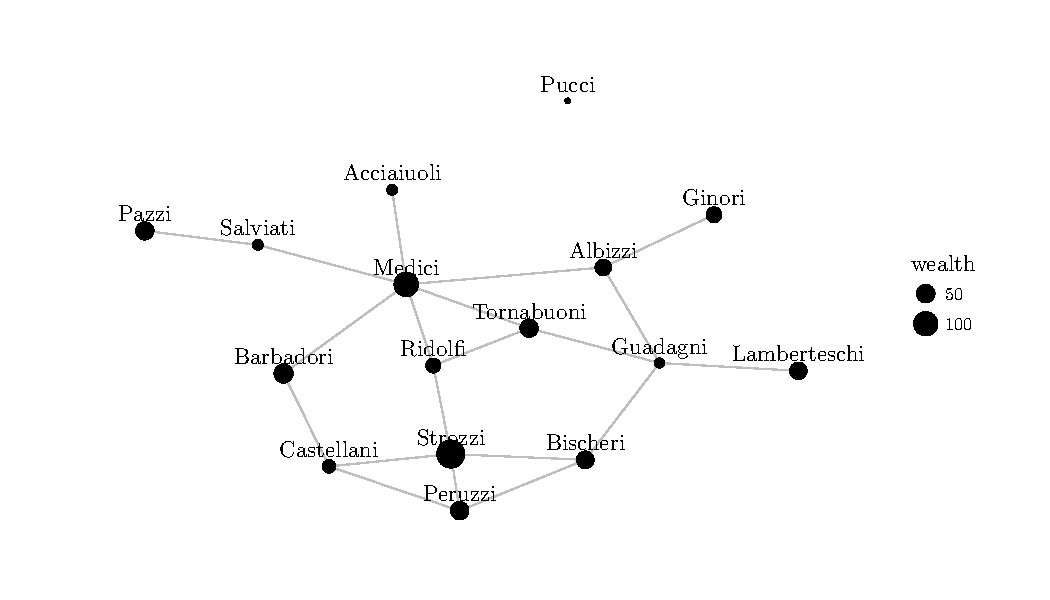
\includegraphics{thesis_files/figure-latex/flo-plot-1} 

}

\caption{A plot of the Florentine marriage network where node size indicates wealth in thousands of lira.}\label{fig:flo-plot}
\end{figure}
For illustrative purposes, we will use the Florentine wedding data
included in the R \texttt{ergm} package by M. S. Handcock et al.
(\protect\hyperlink{ref-Handcock2016a}{2016}), which we also use to fit
MPLE and MCMC-MLE models. We will use the \texttt{Bergm} package by
Caimo \& Friel (\protect\hyperlink{ref-Caimo2014}{2014}) to fit the
Bayesian models. These data consist of an undirected network of
marriages between Florentine families during the Renaissance, along with
several nodal covariates, including the family wealth in thousands of
lira in the year 1427. This network is drawn in Figure
\ref{fig:flo-plot}. We will fit the ERGM with network statistics
\begin{equation}
g(y) = \left( \sum_{i < j} y_{ij}, \sum_{i < j < k} y_{ij} y_{jk} y_{ki}, \sum_{i < j} y_{ij} \left| x_{i} - x_{j} \right| \right),
\label{eq:flo-model}
\end{equation}
where \(y\) is the network and \(x\) is the corresponding vector of
wealth measurements. Simply put, this creates a term for the number of
edges, the number of triangles, and the difference in wealth between
connected nodes in the network. The edge term acts as a sort of
intercept in the model by measuring the overall propensity of actors to
form ties, the triangle term measures the propensity of actors in the
graph to form triangles, and the wealth difference term accounts for how
difference in family fortune affects the probability of tie formation.
Tables \ref{tab:flo-models-mple}, \ref{tab:flo-models-mcmc}, and
\ref{tab:flo-models-bayes} show the coefficient estimates and standard
errors. Bayesian estimation is done using a very flat multivariate
normal prior centered on the origin with variance-covariance matrix
\begin{equation*}
\Sigma = 
\begin{bmatrix}
100 & 0 & 0 \\
0 & 100 & 0 \\
0 & 0 & 100 \\
\end{bmatrix}.
\end{equation*}
Figure \ref{fig:flo-post} shows posterior density estimates for the
Bayesian model.
\begin{table}

\caption{\label{tab:flo-models-mple}The results of fitting model \ref{eq:flo-model} using MPLE.}
\centering
\begin{tabular}[t]{lrr}
\toprule
term & estimate & std.error\\
\midrule
edges & -2.36 & 0.44\\
triangle & 0.16 & 0.44\\
absdiff.wealth & 0.02 & 0.01\\
\bottomrule
\end{tabular}
\end{table}
\begin{table}

\caption{\label{tab:flo-models-mcmc}The results of fitting model \ref{eq:flo-model} using MCMC-MLE.}
\centering
\begin{tabular}[t]{lrr}
\toprule
term & estimate & std.error\\
\midrule
edges & -2.27 & 0.45\\
triangle & -0.04 & 0.59\\
absdiff.wealth & 0.02 & 0.01\\
\bottomrule
\end{tabular}
\end{table}
\begin{table}

\caption{\label{tab:flo-models-bayes}The results of fitting model \ref{eq:flo-model} using Bayesian methods.}
\centering
\begin{tabular}[t]{lrr}
\toprule
term & posterior mean & posterior s.d.\\
\midrule
edges & -2.24 & 0.44\\
triangle & -0.41 & 0.67\\
absdiff.wealth & 0.02 & 0.01\\
\bottomrule
\end{tabular}
\end{table}
\begin{figure}

{\centering 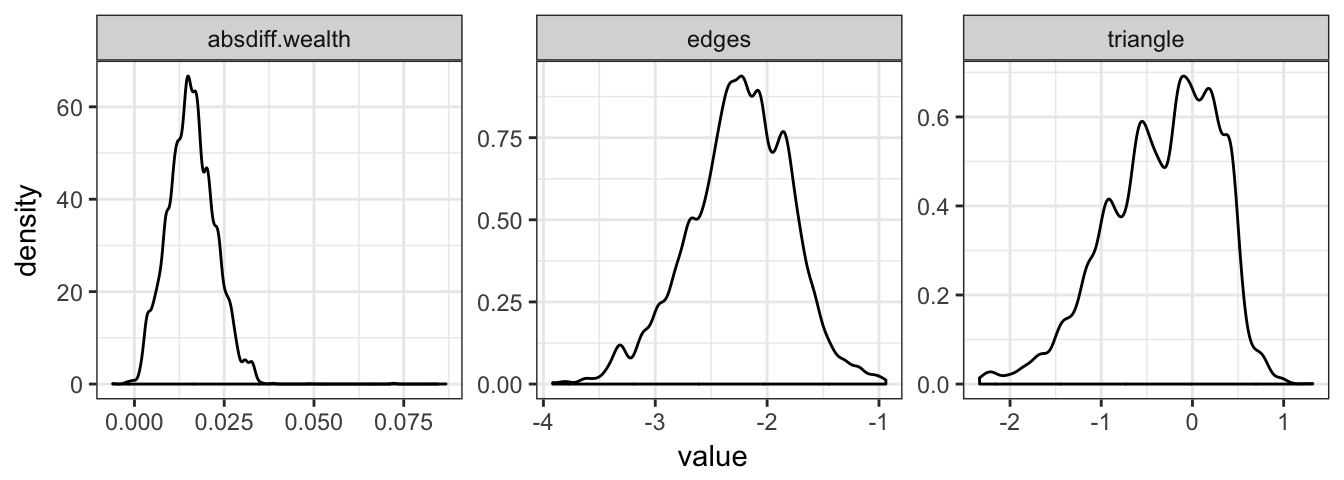
\includegraphics{thesis_files/figure-latex/flo-post-1} 

}

\caption{Posterior density plots of the Florentine marriage model parameter estimates.}\label{fig:flo-post}
\end{figure}
\begin{figure}

{\centering 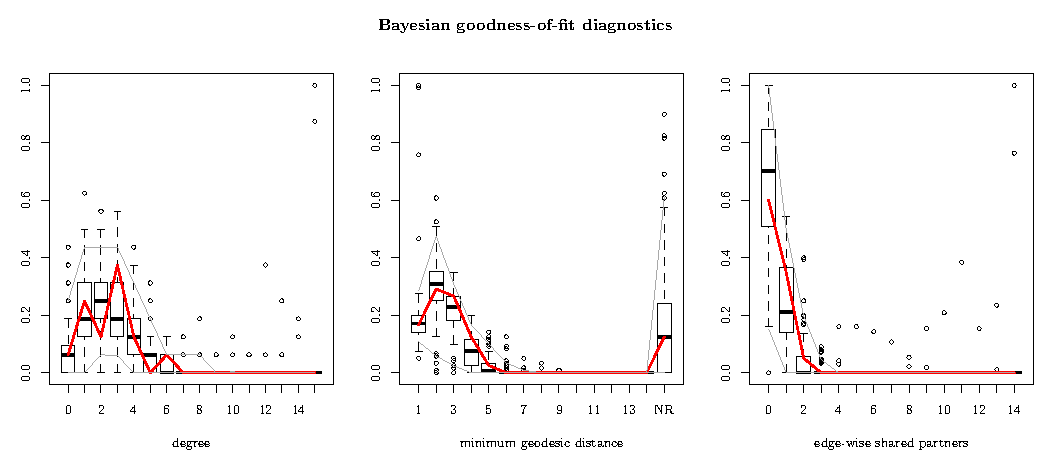
\includegraphics{thesis_files/figure-latex/flo-gof-1} 

}

\caption{Goodness-of-fit assessment for the Bayesian model fit to the Florentine marriage data. These plots compare simulated distributions of graph statistics that were not modeled to the observed values (in red).}\label{fig:flo-gof}
\end{figure}
We can see that all of these methods produce similar outcomes, with a
clearly nonzero edge term, which makes sense as this is akin to an
intercept term in a standard linear model, and a small but significant
term corresponding to the difference in wealth. Notice that the standard
error of the triangle term (which creates dependence between dyads) is
much larger when the model is fit using MCMC-MLE. This supports the
notion that standard errors reported my MPLE are unreliable in dyadic
dependence models, as was discussed in Section
\ref{frequentist-methods}. Interpreting these coefficients allows us to
infer that a difference in wealth of 1 unit (in this case 1000 lira),
changes the log-odds of forming a tie (according to the MCMC-MLE model)
by a factor of \(\theta_3 \approx\) -0.042. The \texttt{ergm} and
\texttt{Bergm} packages also provide tools for assessing the
goodness-of-fit of exponential random graph models. These tools simulate
many networks from the distribution implied by the model with the
parameter estimate and then compare the distributions of several network
statistics that \emph{were not} modeled to the observed network. These
statistics are by default minimum geodesic distance, edgewise shared
partners, and degree distribution. Figure \ref{fig:flo-gof} shows plots
of these comparisons for the Bayesian model. As we can see, our model
matches the simulated distributions fairly well.

\chapter{Locally dependent exponential random network
models}\label{locally-dependent-exponential-random-network-models}
\begin{figure}

{\centering 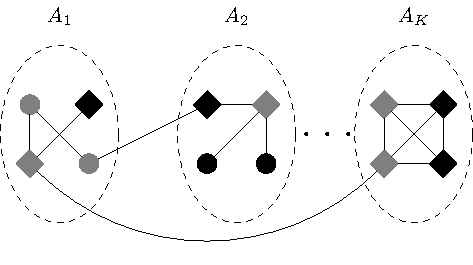
\includegraphics{figure/ld_net} 

}

\caption{A locally dependent random network with neighborhoods \(A_1, A_2, \dots, A_K\) and two binary node attributes, represented as gray or black and circle or diamond.}\label{fig:rn-example}
\end{figure}
To begin, we define a random network, developed by Fellows \& Handcock
(\protect\hyperlink{ref-Fellows2012}{2012}). By way of motivation, note
that in the ERGM the nodal variates are fixed and are included in the
model as explanatory variables in making inferences about network
structure. Furthermore, there is a class of models that we do not
discuss here that consider the network as a fixed explanatory variable
in modeling (random) nodal attributes. It is not difficult to come up
with situations where a researcher would like to \emph{jointly} model
both the network and the node attributes. Thus we define a class of
networks in which both the network structure and the attributes of the
individual nodes are modeled as random quantities.

\BeginKnitrBlock{definition}[Random network]
\protect\hypertarget{def:RN}{}{\label{def:RN} \iffalse (Random network)
\fi{} }Let \(\mathcal{N}\) be a countable collection of nodes (which we
take to be a subset of \(\mathbb{N}\)). Let \(Y\) be the random graph on
the nodes \(\mathcal{N}\) with support \(\mathcal{Y}\). Then for each
element \(n \in \mathcal{N}\), let there be a corresponding random
vector of node attributes \(X_n \in \mathbb{R}^q\) and collect them into
the \(n \times q\) random matrix \(X\) with support \(\mathcal{X}\). The
\emph{random network} is the random variable \(Z = (Y, X)\) with support
\(\mathcal{Z} = \mathcal{Y} \times \mathcal{X}\).
\EndKnitrBlock{definition}

Now we wish to model these objects, so we follow the ERGM and turn to
the exponential family (Fellows \& Handcock,
\protect\hyperlink{ref-Fellows2012}{2012}). We write
\begin{equation}
  P(Y = y, X = x| \eta) \propto e^{\eta \cdot g(y, x)}.
  \label{eq:ERNM}
\end{equation}
This looks very similar to the ERGM, but note the explicit dependence on
the quantity \(x\). More concretely, we can include terms that depend
\emph{only} on \(x\), which would have no place in an ERGM. We can
further express the difference of the two models by rewriting the left
hand side of \ref{eq:ERNM} as
\begin{equation*}
  P(X = x, Y = y | \eta) = P(Y = y|X = x, \eta)P(X=x|\eta),
\end{equation*}
where the first term on the right hand side is the ERGM and the second
term is
\begin{equation*}
  P(X = x|\eta) = \frac{C(\mathcal{Z}, \eta, x)}{C(\mathcal{Z}, \eta)},
\end{equation*}
where
\begin{equation*}
  C(\mathcal{Z}, \eta, x) = \int_{\{(v, u) \in \mathcal{Z} : u = x\}} P(X = x | \eta).
\end{equation*}
Roughly, this is the proportion of the total sample space
\(\mathcal{Z}\) that is possible with \(x\) fixed. This is not, in
general, equal to one, so the ERNM is not equal to the ERGM (Fellows \&
Handcock, \protect\hyperlink{ref-Fellows2012}{2012}).

\section{Definitions and notation}\label{definitions-and-notation}

We will consistently refer to a set of nodes, \(A_{k}\), as the \(k\)-th
neighborhood, with an uppercase \(K\) representing the total number of
neighborhoods and a lowercase \(k\) representing a specific
neighborhood. The variable \(\mathcal{N}\) will refer to the domain of a
random network, usually the union of a collection of neighborhoods.
Nodes within the network will be indexed by the variables \(i\) and
\(j\), with \(Z_{ij} = (\{Y_{ij}, X_i, X_j\})\), where \(Y_{ij}\) is
referring to the edge between nodes \(i\) and \(j\), and \(X_{i}\) and
\(X_j\) refer to the random vectors of node attributes. Abstracting this
further, \(i\) and \(j\) will also refer to tuples of nodes, so we will
write
\(\vec{i} = (i_1, i_2, \dots, i_q) \in \mathcal{N} \times \mathcal{N} \times \dots \times \mathcal{N}\).
The variables \(Z\) and \(Y\) will also often carry a subscript of \(W\)
or \(B\) (for example \(Y_{Bij}\)) which emphasizes that the edge from
\(i\) to \(j\) is within or between neighborhoods, respectively.
Finally, for lack of a better notation, the indicator function
\(\mathbb{I}_{B}(i,j)\) (where \(B\) is for between) is one if
\(i \in A_{l}\) and \(j \in A_{p}\) where \(l \neq p\), and zero
otherwise.

\BeginKnitrBlock{definition}[Local dependence property]
\protect\hypertarget{def:unnamed-chunk-1}{}{\label{def:unnamed-chunk-1}
\iffalse (Local dependence property) \fi{} }Extending the definition in
Schweinberger \& Handcock
(\protect\hyperlink{ref-Schweinberger2015}{2015}), a random network
model satisfies \emph{the local dependence property} if there is a
partition of the node set \(\mathcal{N}\) into neighborhoods
\(A_1, A_2, \dots, A_K\) for \(K \geq 2\) such that the network
variables \(Z_{ij}\) are dependent when \(i, j \in A_{\ell}\) for some
\(\ell\) and independent otherwise. We also require that nodal
attributes depend only on the attributes of nodes within the same
neighborhood. Thus, the probability measure can be written as
\begin{equation}
    P(Z \in \mathbf{Z}) = \prod_{k = 1}^{K}\left[ P_{kk}(Z_{kk} \in \mathbf{Z}_{kk}) \prod_{\ell = 1}^{k-1} P_{kl}(Z_{kl} \in \mathbf{Z}_{kl}, Z_{lk} \in \mathbf{Z}_{lk}) \right],
  \end{equation}
where \(Z_{mn}\) is the subnetwork consisting of the random graph ties
from nodes in \(A_m\) to those in \(A_n\) and the appropriate node
variables and \(\mathbf{Z}_{mn}\) is a subset of the sample space of
\(Z_{mn}\). Furthermore, the measures \(P_{kk}\) can induce dependence
between dyads while the measures \(P_{kl}\) induce independence.
\EndKnitrBlock{definition}

\BeginKnitrBlock{definition}[Sparsity]
\protect\hypertarget{def:unnamed-chunk-2}{}{\label{def:unnamed-chunk-2}
\iffalse (Sparsity) \fi{} }Also from Schweinberger \& Handcock
(\protect\hyperlink{ref-Schweinberger2015}{2015}), we say a locally
dependent random network is \emph{\(\delta\)-sparse} if there is some
\(\delta > 0\) and some \(C > 0\) such that
\begin{equation}
    \mathbb{E}\left( \left| Y_{Bij} \right|^{p} \right) \leq Cn^{-\delta}, \qquad (p = 1, 2)
  \end{equation}
where \(n = |\mathcal{N}|\) and \(Y_{Bij}\) signifies the tie between
neighborhoods from node \(i \in A_{l}\) to node \(j \in A_{m}\) where
\(l \neq m\).
\EndKnitrBlock{definition}

\section{Preliminary theorems}\label{preliminary-theorems}

In proving our theorems, we will make use of several other central limit
theorems, all of which can be found in Billingsley
(\protect\hyperlink{ref-Billingsley1995}{1995}). The first is the
Lindeberg-Feller central limit theorem for triangular arrays. The second
is Lyapounov's condition, which gives a convenient way to show that the
Lindeberg-Feller theorem holds. Finally, we make use of a central limit
theorem for dependent random variables. For the sake of brevity, in this
section we state each of these without proof.

\BeginKnitrBlock{theorem}[Billingsley, 1995 Theorem 27.2]
\protect\hypertarget{thm:unnamed-chunk-3}{}{\label{thm:unnamed-chunk-3}
\iffalse (Billingsley, 1995 Theorem 27.2) \fi{} }For each \(n\) take
\(X_{n1}, \dots, X_{nr_n}\), independent with \(\mathbb{E}(X_{ns}) = 0\)
for all \(n\) and \(s\) (where no generality is lost in this
assumption). Then we have
\(\sigma^{2}_{ns} = \operatorname{Var}(X_{ns}) = \mathbb{E}(X_{ns}^2)\).
Next, set \(s^{2}_{s} = \sum_{s = 1}^{r_n} \sigma^{2}_{ns}\). Now set
\begin{equation*}
S_{n} = X_{n1} + \dots + X_{nr_n}.
\end{equation*}
If the \emph{Lindeberg condition},
\begin{equation}
\lim_{n \to \infty} \sum_{s = 1}^{r_n} \frac{1}{s^{2}_{n}} \int_{|X_{ns} \geq \epsilon s_n} X^{2}_{ns} = 0
\end{equation}
holds for all \(\epsilon > 0\), then
\(S_n \xrightarrow{\mathrm{d}} N(0,1)\).
\EndKnitrBlock{theorem}

\BeginKnitrBlock{theorem}[Billingsley, 1995 Theorem 27.3]
\protect\hypertarget{thm:unnamed-chunk-4}{}{\label{thm:unnamed-chunk-4}
\iffalse (Billingsley, 1995 Theorem 27.3) \fi{} }Let \(S_n\) be as
before. Then if \emph{Lyapounov's condition},
\begin{equation}
\lim_{n \to \infty} \sum_{s = 1}^{r_n} \frac{1}{s_n^{2 + \delta}} \mathbb{E} \left( \left| X_{ns} \right|^{s + \delta} \right) = 0
\label{eq:lya}
\end{equation}
holds for some \(\delta > 0\), then the Lindeberg condition also holds.
Therefore \(S_{n} \xrightarrow{\mathrm{d}} N(0,1)\).
\EndKnitrBlock{theorem}

\BeginKnitrBlock{theorem}[Billingsley, 1995 Theorem 27.4]
\protect\hypertarget{thm:unnamed-chunk-5}{}{\label{thm:unnamed-chunk-5}
\iffalse (Billingsley, 1995 Theorem 27.4) \fi{} }Suppose that
\(X_1, X_2, \dots\) is stationary and \(\alpha\)-mixing with
\(\alpha_n = O(n^{-5})\) and that \(\mathbb{E}(X_n) = 0\) and
\(\mathbb{E}(X_n^{12}) < \infty\). Note that the condition on \(\alpha\)
is stronger than what we require. Our \(X_n\) will be \(M\)-dependent,
meaning that each \(X_n\) is independent of all \(X_m\) where
\(|n - m| > M\). It is true that an \(M\)-dependent sequence is
\(\alpha\)-mixing for constant \(\alpha\). Then, if
\(S_n = X_1 + \dots X_n\), we have
\begin{equation}
\frac{\operatorname{Var}(S_n)}{n} \to \sigma^2.
\end{equation}
Then, if \(\sigma > 0\), we have
\(S_n \xrightarrow{\mathrm{d}} N(0,1)\).
\EndKnitrBlock{theorem}

The final theorem is Slutsky's theorem, a classic result of asymptotic
theory in statistics.

\BeginKnitrBlock{theorem}[Wasserman, 2004 Theorem 5.5]
\protect\hypertarget{thm:slutsky}{}{\label{thm:slutsky} \iffalse (Wasserman,
2004 Theorem 5.5) \fi{} }Let \(X_n, X, Y_n\) be random variables and let
\(c\) be a constant. Then, if \(X_n \xrightarrow[]{\mathrm{d}} X\) and
\(Y \xrightarrow[]{\mathrm{p}} c\) we have
\(X_n + Y_n \xrightarrow[]{\mathrm{d}} X + c\) and
\(X_n Y_n \xrightarrow[]{\mathrm{d}} cX\).
\EndKnitrBlock{theorem}

\section{Consistency under sampling}\label{consistency-under-sampling}

With these in place, we attempt to extend a result about locally
dependent ERGMs proven by Schweinberger \& Handcock
(\protect\hyperlink{ref-Schweinberger2015}{2015}) to locally dependent
ERNMs. In short, this theorem states that the parameters estimated by
modeling a small sample of a larger network can be generalized to the
overall network. It was shown by Shalizi \& Rinaldo
(\protect\hyperlink{ref-Shalizi2013}{2013}) that most useful
formulations of ERGMs do not form projective exponential families in the
sense that the distribution of a subgraph cannot be, in general,
recovered by marginalizing the distribution of a larger graph with
respect to the edge variables not included in the smaller graph. Hence,
we are unable to generalize parameter estimates from the subnetwork to
the total network.

To show that locally dependent ERNMs do form a projective family, let
\(\mathbb{A}\) be a collection of sets \(\mathcal{A}\), where each
\(\mathcal{A}\) is a finite collection of neighborhoods. Also, allow the
set \(\mathbb{A}\) to be an ideal, so that if
\(\mathcal{A} \in \mathbb{A}\), every subset of \(\mathcal{A}\) is also
in \(\mathbb{A}\) and if \(\mathcal{B} \in \mathbb{A}\), then
\(\mathcal{A} \cup \mathcal{B} \in \mathbb{A}\). If
\(\mathcal{A} \subset \mathcal{B}\), think of passing from the set
\(\mathcal{A}\) to the set \(\mathcal{B}\) as taking a larger sample of
the (possibly infinite) set of neighborhoods in the larger network. Then
let
\(\{\mathcal{P}_{\mathcal{A}, \theta}\}_{\mathcal{A} \in \mathbb{A}}\)
be the collection of ERNMs with parameter \(\theta\) indexed by the sets
in \(\mathbb{A}\). For each \(\mathcal{A} \in \mathbb{A}\), let
\(\mathcal{P}_{\mathcal{A}, \Theta} = \{P_{\mathcal{A}, \theta}\}_{\theta \in \Theta}\)
be the collection of ERNMs on the neighborhoods in \(\mathcal{A}\) with
parameter \(\theta \in \Theta\) where \(\Theta \subset \mathbb{R}^{p}\)
is open. Assume that each distribution in
\(\mathcal{P}_{\mathcal{A}, \Theta}\) has the same support
\(\mathcal{Z}_{\mathcal{A}}\) and that
\(\mathcal{A} \subset \mathcal{B}\) if and only if
\(\mathcal{Z}_{\mathcal{B}} = \mathcal{Z}_{\mathcal{A}} \times \mathcal{Z}_{\mathcal{B} \setminus \mathcal{A}}\).
Then, the exponential family
\(\{\mathcal{P}_{\mathcal{A}, \Theta}\}_{\mathcal{A} \in \mathbb{A}}\)
is projective in the sense of Shalizi \& Rinaldo
(\protect\hyperlink{ref-Shalizi2013}{2013} Definition 1) precisely when
Theorem \ref{thm:consistency} holds.

This follows from a specific case of the general definition given by
Shalizi \& Rinaldo (\protect\hyperlink{ref-Shalizi2013}{2013}). There,
for every pair \(\mathcal{A}\) and \(\mathcal{B}\) with
\(\mathcal{A} \subset \mathcal{B}\), they define the natural projection
mapping
\(\pi_{\mathcal{B} \to \mathcal{A}}: \mathcal{Z_B} \to \mathcal{Z_A}\).
Informally, this mapping projects the set \(\mathcal{Z_B}\) down to
\(\mathcal{Z_A}\) by simply removing the extra data. For example if
\(\mathcal{B} = \{A_1, A_2\}\) and \(\mathcal{A} = \{A_1\}\) as in
Figure \ref{fig:rn-example}, then the mapping
\(\pi_{\mathcal{B} \to \mathcal{A}}\) is shown in Figure
\ref{fig:net-proj}.
\begin{figure}

{\centering 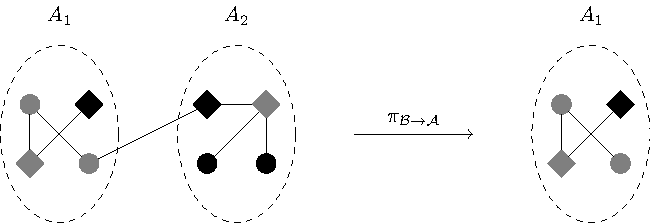
\includegraphics{figure/net_projection} 

}

\caption{The projection mapping from \(\mathcal{B} = \{A_1, A_2\}\) to \(\mathcal{A} = \{A_1\}\).}\label{fig:net-proj}
\end{figure}
This is desirable because Shalizi \& Rinaldo
(\protect\hyperlink{ref-Shalizi2013}{2013}) have demonstrated the
following theorem.

\BeginKnitrBlock{theorem}[Shalizi \& Rinaldo, 2013 Theorem 3]
\protect\hypertarget{thm:unnamed-chunk-6}{}{\label{thm:unnamed-chunk-6}
\iffalse (Shalizi \& Rinaldo, 2013 Theorem 3) \fi{} }If the exponential
model family
\(\{\mathcal{P}_{\mathcal{A} \Theta}\}_{\mathcal{A} \in \mathbb{A}}\) is
projective and the log of the normalizing constant can be written as
\begin{align}
\begin{split}
\log \left( C(\theta, \mathcal{Z}) \right) &= \log \left( \int_{\mathcal{Z}} e^{\theta \cdot g(z)} \;\mathrm{d}z \right) \\
                                          &= r \left(\left| \mathcal{Z} \right| \right) a(\theta),
\end{split}
\end{align}
where \(r\) is a positive, monotone increasing function of some positive
measure on \(\mathcal{Z}\) and \(a\) is a differentiable function of
\(\theta\), then the maximum likelihood estimator exists and is strongly
consistent, meaning that the MLE,
\(\hat{\theta} \xrightarrow[]{\text{a.s.}} \theta\), where \(\theta\) is
the unknown parameter being estimated.
\EndKnitrBlock{theorem}

This is trivially achieved by setting \(r = 1\) for all values of
\(\left| \mathcal{Z} \right|\) and setting
\(a(\theta) = \log(C(\theta, \mathcal{Z}))\). We have differentiability
of \(a\) with respect to \(\theta\) by a result from multivariable
calculus that follows from Fubini's theorem. From a practical
perspective, this means that a researcher using this model can assume
that parameters estimated from samples of a large network are
increasingly good approximations for the true parameter values as the
sample size increases.

\BeginKnitrBlock{theorem}
\protect\hypertarget{thm:consistency}{}{\label{thm:consistency}}Let
\(A_{1}, A_{2}, \dots\) be a sequence of neighborhoods and define the
sequence \(\{\mathcal{N}_{K}\} = \bigcup_{i = 1}^{K} A_{i}\). Then let
\(Z_{1}, Z_{2}, \dots\) be the sequence of locally dependent random
networks on the \(\mathcal{N}_K\). For each \(Z_K\), there is the
corresponding set of neighborhoods \(\mathcal{A}_K\). Let \(P_K\) be a
generic probability distribution from the family
\(\{\mathcal{P}_{K \theta}\}_{\theta \in \Theta}\). Let the network
\begin{equation*}
\pi_{\mathcal{A}_{K+1} \to \mathcal{A}_K}(Z_{K+1}) = Z_{K+1 \setminus K},
\end{equation*}
with corresponding distirbution \(P_{K+1 \setminus K}\). Then
\begin{equation}
    P_{K}(Z_{K} \in \mathbf{Z}_K) = P_{K+1}(Z_{K} \in \mathbf{Z}_K, Z_{K+1 \setminus K} \in \mathcal{Z}_{K+1 \setminus K}),
  \end{equation}
my\_dev where \(\mathcal{Z}_K\) is the sample space of the distribution
\(P_{K}\) and \(\mathbf{Z}_K \subset \mathcal{Z}_K\). This is a specific
case of the definition of projectibility for a general exponential
family given by Shalizi \& Rinaldo
(\protect\hyperlink{ref-Shalizi2013}{2013}).
\EndKnitrBlock{theorem}

\BeginKnitrBlock{proof}
\iffalse {Proof. } \fi{} This follows from the definition of local
dependence, in much the same way as the proof for ERGMs by Schweinberger
\& Handcock (\protect\hyperlink{ref-Schweinberger2015}{2015}) does. We
have
\begin{align*}
    P_{K+1}(Z_{K} \in \mathbf{Z}_K, Z_{K+1 \setminus K} \in \mathcal{Z}_{K+1 \setminus K}) &= P_{K+1}(Z_{K} \in \mathbf{Z}_K) P_{K+1 \setminus K}(Z_{K+1 \setminus K} \in \mathcal{Z}_{K+1 \setminus K}) \\
    &= P_{K}(Z_{K} \in \mathbf{Z}_K) (1) \\
    &= P_{K}(Z_{K} \in \mathbf{Z}_K),
  \end{align*}
where the measure becomes \(P_k\) from the product definition of a
locally dependent random network. \qedhere
\EndKnitrBlock{proof}

\section{Asymptotic normality of
statistics}\label{asymptotic-normality-of-statistics}

In this section we will prove that certain classes of statistics of
locally dependent random networks are asymptotically normally
distributed as the number of neighborhoods tends to infinity. The
statistics we consider can be classified into three types: first,
statistics which depend only on the graph structure; second, statistics
that depend on both the graph and the nodal variates; and third,
statistics that depend only on the nodal variates. The first class of
statistics has already been considered by Schweinberger \& Handcock
(\protect\hyperlink{ref-Schweinberger2015}{2015}), but we will reproduce
the proof here, as the second proof is very similar. The third class of
statistics becomes normal in the limit by a central limit theorem for
\(M\) dependent random variables in Billingsley
(\protect\hyperlink{ref-Billingsley1995}{1995}).

Before we begin to explicitly define each of these classes, we clarify
the notation that will be used. A general statistic will be a function
\begin{equation*}
S:\mathcal{N}^d \to \mathbb{R},
\end{equation*}
where \(\mathcal{N}^d\) is the \(d\)-fold Cartesian product of the set
of nodes, \(\mathcal{N}\), with itself:
\begin{equation*}
\mathcal{N}^d = \underbrace{\mathcal{N} \times \dots \times \mathcal{N}}_{d \text{ times}}.
\end{equation*}
Additionally, the statistic will often carry a subscript \(K\),
indicating that the statistic is of the random network with \(K\)
neighborhoods.

Formally, as explained in Schweinberger \& Handcock
(\protect\hyperlink{ref-Schweinberger2015}{2015}), the first class of
statistics contains those that have the form
\begin{equation*}
S_{K} = \sum_{i \in \mathcal{N}^d} S_{Ki},
\end{equation*}
where
\begin{equation*}
S_{Ki} = \prod_{l, p \in i} Y_{lp}, 
\end{equation*}
a product \(q\) of edge variables that captures the interaction desired.
We will also make use of the set \(A_k^d,\) wich is a similar cartesian
product. When we write \(i \in A_k^d\), we mean the every component of
the \(d\)-tuple \(i\) is an element of \(A_k\). Furthermore, by a
catachrestic abuse of notation, we will write \(l, p \in i\) to mean
that \(l\) and \(p\) are vertices contained in the \(d\)-tuple \(i\).
Now we are ready to prove the first case of the theorem.

\BeginKnitrBlock{theorem}
\protect\hypertarget{thm:norm1}{}{\label{thm:norm1}}Let
\(A_1, A_2, \dots, A_K\) be a sequence of neighborhoods of size at most
\(M\) and form the sequence of domains
\(\mathcal{N}_{K} = \bigcup_{k = 1}^{K} A_{k}\). Then let
\(Z_{1}, Z_{2}, \dots, Z_{K}\) be the sequence of unweighted random
networks on the \(\mathcal{N}_{K}\). Then, let the statistic
\(S_{K}:\mathcal{N}_{K}^d \to \mathbb{R}\) be given. Furthermore, assume
the statistic depends only on the graph variables of the \(Z_{K}\). We
also assume that the \(Z_{K}\) satisfy the local dependence property and
that they are \(\delta\)-sparse, for some \(\delta > d\). Finally, we
require that \(\operatorname{Var}(W^{\ast}_{K}) \to \infty\), where
\(W^{\ast}_{K}\) is defined in \eqref{eq:WK-def}. Then
\begin{equation}
\frac{S_K - \mathbb{E}(S_K)}{\sqrt{Var(S_{K})}} \xrightarrow[K \to \infty]{\mathrm{d}} N(0, 1).
\end{equation}
\EndKnitrBlock{theorem}

\BeginKnitrBlock{proof}
\iffalse {Proof. } \fi{} As the networks \(Z_K\) are unweighted, all
edge variables \(Y_{ij}\in \{0, 1\}\). Let
\(\mu_{ij} = \mathbb{E}(Y_{ij})\). Then define
\(V_{ij} = Y_{ij} - \mu_{ij}\). Therefore, without loss of generality,
we may work with \(V_{ij}\), which has the convenient property that
\(\mathbb{E}(V_{ij}) = 0\). This means that we can similarly shift our
statistics of interest, \(S_K\). Therefore, call
\(S_K^{\ast} = S_{K} - \mathbb{E}(S_K)\), so that
\(\mathbb{E}(S_K^{\ast}) = 0\).

Note that we can write
\begin{equation*}
  S^{\ast}_{K} = W^{\ast}_{K} + B^{\ast}_{K},
\end{equation*}
with
\begin{equation}
  W^{\ast}_{K} = \sum_{k = 1}^{K} W^{\ast}_{K,k} = \sum_{k = 1}^{K}  \sum_{i \in \mathcal{N}_{K}^d} \mathbb{I}(i\in A_{k}^d) S^{\ast}_{Ki}
  \label{eq:WK-def}
\end{equation}
and
\begin{equation}
  B^{\ast}_{K} = \sum_{i \in \mathcal{N}_{K}^d} \mathbb{I}_{B}(i) S^{\ast}_{Ki},
\end{equation}
where the indicator functions restrict the sums to within the \(k\)-th
neighborhood and between neighborhoods of the graph, respectively.
Specifically, \(\mathbb{I}_{B}(i) = 1\) when the \(d\)-tuple of nodes
\(i\) contains nodes from different neighborhoods, or exactly when
\(\mathbb{I}(i \ in A_{k}^d) = 0\) for all neighborhoods \(k\). By
splitting the statistic into the within and between neighborhood
portions, we are able to make use of the independence relation between
edges that connect neighborhoods. We also have
\(\mathbb{E}(W^{\ast}_{K}) = 0\) and \(\mathbb{E}(B^{\ast}_{K}) = 0\),
as each quantity is a sum of random variables with mean zero.

The idea of this proof is to gain control over the variances of
\(B^{\ast}_{K}\) and all the elements of the sequence \(W^{\ast}_{Kk}\).
We can then show that \(B^{\ast}_{K}\) is converging in probability to
zero and that the triangular array \(W^{\ast}_{K}\) satisifies
Lyaponouv's condition, and is thus asymptotically normal. Finally,
Slutsky's theorem allows us to extend the result to \(S^{\ast}_{K}\).

To bound the variance of \(B^{\ast}_{K}\), note that
\begin{equation*}
\operatorname{Var}(B^{\ast}_{K}) = \sum_{i \in \mathcal{N}_{K}^d} \sum_{j \in \mathcal{N}_{K}^d} \mathbb{I}_{B}(i) \mathbb{I}_{B}(j) \operatorname{Cov}(S^{\ast}_{Ki}, S^{\ast}_{Kj}).
\end{equation*}
Despite independence, some of these covariances may be nonzero if the
two terms of the statistic both involve the same edge. For example, in
Figure \ref{fig:rn-example}, a statistic that counted the number of
edges between gray nodes plus the number of edges between diamond shaped
nodes would have a nonzero covariance term because of the edge between
the two nodes that are both gray and diamond shaped. To show that, in
the limit, these covariances vanish, we need only concern ourselves with
the nonzero terms in the sum. That is, only those terms where
\(\mathbb{I}_{B}(i) \mathbb{I}_{B}(j) = 1\). This happens exactly when
both \(S^{\ast}_{Ki}\) and \(S^{\ast}_{Kj}\) involve a between
neighborhood edge variable. So, note that we have
\begin{align}
  \begin{split}
  \operatorname{Cov}(S^{\ast}_{Ki}, S^{\ast}_{Kj}) &= \mathbb{E}(S^{\ast}_{Ki} S^{\ast}_{Kj}) - \mathbb{E}(S^{\ast}_{Ki}) \mathbb{E}(S^{\ast}_{Kj}) \\
  &= \mathbb{E}(S^{\ast}_{Ki}S^{\ast}_{Kj}),
\end{split}
\end{align}
as the expectation of each term is zero. Next we take \(Y_{l_1 l_2}\) to
be one of the (possibly many) between neighborhood edge variables in
this product (such that \(\mathbb{I}_B(i) = 1\) where \(i\) is any tuple
containing \(l_1\) and \(l_2\)) and \(V_{l_1 l_2}\) to be the recentered
random variable corresponding to \(Y_{l_1 l_2}\). Then,
\begin{align*}
\operatorname{Cov}(S^{\ast}_{Ki}, S^{\ast}_{Kj}) &= \mathbb{E}\left( \prod_{m,n \in i} V_{mn} \prod_{m,n \in j} V_{mn} \right) \\
                     &= \mathbb{E}\left( V_{l_1 l_2}^p \prod_{m,n \in (i \cup j) \setminus \{l_1, l_2\}} V_{mn} \right), & (p = 1,2)
\end{align*}
where we must consider the case where \(p = 1\) to account for the
covariance of \(S^{\ast}_{Ki}\) and \(S^{\ast}_{Kj}\) when \(i \neq j\)
and the case where \(p = 2\) to account for the variance of
\(S^{\ast}_{Ki}\), which is computed in the case where \(i = j\). So, if
\(p = 1\), then
\begin{align*}
\mathbb{E}\left( V_{l_1 l_2} \prod_{m,n \in (i \cup j) \setminus \{l_1, l_2\}} V_{mn} \right) &= \mathbb{E}\left( V_{l_1 l_2}\right) \mathbb{E}\left( \prod_{m,n \in (i \cup j) \setminus \{l_1, l_2\}} V_{mn} \right) \\
&= 0,
\end{align*}
by the local dependence property and the assumption that
\(\mathbb{E}(V_{l_1 l_2}) = 0\). The local dependence property allows us
to factor out the expectation of \(V_{l_1 l_2}\), as this edge is
between neighborhoods, and therefore independent of every other edge in
the graph. Now, if we have \(p = 2\), then, by sparsity and the fact
that the product below is at most \(1\),
\begin{equation*}
\mathbb{E}\left( V_{l_1 l_2}^2\right) \mathbb{E}\left( \prod_{m,n \in (i \cup j) \setminus \{l_1, l_2\}} V_{mn} \right) \leq DCn^{-\delta},
\end{equation*}
where D is a constant that bounds the expectation above. There exists
such a constant because each of the V\_\{mn\} are bounded by definiton,
so a product of them is bounded. So as \(K\) grows large, the between
neighborhod covariances all become asymptotically negligible. Therefore,
we can conclude that
\begin{equation}
\operatorname{Var}(B^{\ast}_{K}) = \sum_{i \in \mathcal{N}_{K}^d} \sum_{j \in \mathcal{N}_{K}^d} \mathbb{I}_{B}(i) \mathbb{I}_{B}(j) \operatorname{Cov}(S^{\ast}_{Ki}, S^{\ast}_{Kj}) \leq DCn^{2d(-\delta)}.
\end{equation}
So we have
\begin{equation}
\operatorname{Var}{B^{\ast}_{K}} \to 0.
\end{equation}
Then, for all \(\epsilon > 0\), Chebyshev's inequality gives us
\begin{equation}
  \lim_{K \to \infty} P(|B^{\ast}_{K}| > \epsilon) \leq \lim_{K \to \infty} \frac{1}{\epsilon^2} \operatorname{Var}(B^{\ast}_{K}) = 0,
\end{equation}
so
\begin{equation}
  B^{\ast}_{K} \xrightarrow[K \to \infty]{\text{p}} 0.
\end{equation}
Next, we bound the within neighborhood covariances, as we also have
\begin{equation*}
\operatorname{Var}(W^{\ast}_{Kk}) = \sum_{i \in \mathcal{N}_{K}^d} \sum_{j \in \mathcal{N}_{K}^d} \mathbb{I}(i, j \in A_{k})  \operatorname{Cov}(S^{\ast}_{Ki}, S^{\ast}_{Kj}).
\end{equation*}
As the covariance forms an inner product on the space of square
integrable random variables, the Cauchy-Schwarz inequality gives us
\begin{equation}
  \mathbb{I}(i, j \in A_{k}) \left| \operatorname{Cov}(S^{\ast}_{Ki}, S^{\ast}_{Kj}) \right| \leq \mathbb{I}(i, j \in A_{k}) \sqrt{\operatorname{Var}(S^{\ast}_{Ki})} \sqrt{\operatorname{Var}(S^{\ast}_{Kj})}.
\end{equation}
Then, as each \(S^{\ast}_{Ki}\) has expectation zero, we know that
\begin{equation}
  \operatorname{Var}(S^{\ast}_{Ki}) = \mathbb{E}(S^{\ast 2}_{Ki}) - \mathbb{E}(S^{\ast}_{Ki})^2 = \mathbb{E}(S^{\ast 2}_{Ki}).
\end{equation}
As \(S^{\ast 2}_{Ki} \leq 1\), we know
\(\operatorname{Var}(S^{\ast}_{Ki}) \leq 1\) for all tuples \(i\), so we
have the bound
\begin{equation}
  \mathbb{I}(i, j \in A_{k}) \left| \operatorname{Cov}(S^{\ast}_{Ki}, S^{\ast}_{Kj}) \right| \leq  \mathbb{I}(i, j \in A_{k}).
\end{equation}
Now all that remains is to apply the Lindeberg-Feller central limit
theorem to the double sequence
\(W^{\ast}_{K} = {\sum_{k = 1}^{K} W^{\ast}_{K, k}}\). To that end,
first note that, as each neighborhood contains at most a finite number
of nodes, \(M\), we can show that
\begin{align}
    \begin{split}
    \operatorname{Var}(W^{\ast}_{K,k}) &= \sum_{i \in \mathcal{N}_{K}^d} \sum_{j \in \mathcal{N}_{K}^d} \mathbb{I}(i,j \in A_k^d) \operatorname{Cov}(S^{\ast}_{Ki}, S^{\ast}_{Kj}) \\
    &= \sum_{i \in \mathcal{N}_{K}^d} \sum_{j \in \mathcal{N}_{K}^d} \mathbb{I}(i,j \in A_k^d) \mathbb{E}(S^{\ast}_{Ki} S^{\ast}_{Kj}) \\
    &\leq \sum_{i \in \mathcal{N}_{K}^d} \sum_{j \in \mathcal{N}_{K}^d} 1 \\
    &\leq M^{2d}.
  \end{split}
\end{align}
Now we prove that Lyaponouv's condition \eqref{eq:lya} holds for the
constant in the exponent \(\delta = 2\). So
\begin{align}
    \begin{split}
    \lim_{K \to \infty} \sum_{k = 1}^{K} \frac{1}{\operatorname{Var}(W^{\ast}_{K})^2} \mathbb{E}(|W^{\ast}_{K,k}|^{4}) &= \lim_{K \to \infty} \frac{1}{\operatorname{Var}(W^{\ast}_{K})^2} \sum_{k = 1}^{K}  \mathbb{E}(W^{\ast 2}_{K,k}) \mathbb{E}(W^{\ast 2}_{K,k}) \\
    &\leq \lim_{K \to \infty} \frac{M^{2d}}{\operatorname{Var}(W^{\ast}_{K})^2} \sum_{k = 1}^{K} \mathbb{E}(W^{\ast}_{K,k})^2 \\
    &= \lim_{K \to \infty} \frac{M^{2d}}{\operatorname{Var}(W^{\ast}_{K})^2} \sum_{k = 1}^{K} \operatorname{Var}(W^{\ast}_{K,k}) \\
    &= \lim_{K \to \infty} \frac{M^{2d}}{\operatorname{Var}(W^{\ast}_{K})} \\
    &= 0.
  \end{split}
  \label{eq:lya}
\end{align}
where \(\operatorname{Var}(W^{\ast}_{K})\) tends to infinity by
assumption. Therefore, Lyaponouv's condition holds, and so by the
Lindeberg-Feller central limit theorem, we have,
\begin{equation}
  \frac{W^{\ast}_K}{\sqrt{\operatorname{Var}(W^{\ast}_K)}} \xrightarrow[K \to \infty]{\text{d}} N(0, 1).
\end{equation}
Slutsky's theorem (\ref{thm:slutsky}) gives the final result for
\(S^{\ast}_{K} = W^{\ast}_{K} + B^{\ast}_{K}\). Then we have
\begin{equation}
  \frac{S^{\ast}_K}{\sqrt{\operatorname{Var}(S^{\ast}_K)}} \xrightarrow[K \to \infty]{\text{d}} N(0, 1),
\end{equation}
as desired.\qedhere
\EndKnitrBlock{proof}

The second class of statistics are those that depend on both the graph
and the nodal variates. These have a very similar form as the statistics
previously considered. Now we require that
\begin{equation*}
S_{K} = \sum_{i \in \mathcal{N}^d} S_{Ki},
\end{equation*}
where
\begin{equation*}
S_{Ki} = \prod_{l,p \in i} Y_{lp} h(X_l, X_p),
\end{equation*}
a product with at most \(q\) terms.

\BeginKnitrBlock{theorem}
\protect\hypertarget{thm:unnamed-chunk-9}{}{\label{thm:unnamed-chunk-9}}If
\(S_K\) is a statistic depending on both the random graph and the random
nodal attributes, the sequence of random networks are as before, and the
function \(h\) is uniformly bounded in the sense that, for all \(l\) and
\(m\), there is some \(B\) such that
\begin{equation*}
P \left( |h(X_l, X_m)|^p > B \right) = 0, \qquad (p = 1, 2)
\end{equation*}
then we also have
\begin{equation*}
S_{K} \xrightarrow[K \to \infty]{\mathrm{d}} N(0,1).
\end{equation*}
\EndKnitrBlock{theorem}

\BeginKnitrBlock{proof}
\iffalse {Proof. } \fi{} This proof is very similar to the proof of
Theorem \ref{thm:norm1}. We write
\begin{equation*}
S_{K} = W{K} + B{K},
\end{equation*}
exactly as before, incorporating the function \(h\) into each \(S_{Ki}\)
as we did above. Then the binary nature of the graph and the uniform
boundedness of \(h\) allow us to once again recenter the \(Y_{ij}\),
meaning that we will work with
\(V_{ij}h(X_i, X_j) = Y_{ij}h(X_i, X_j) - \mu_{ij}\). We also have
\(\mathbb{E}(V_{ij} h(X_i, X_j)) = 0\), so
\(\mathbb{E}(S^{\ast}_{Ki}) = 0\) as well.

For the between neighborhood covariances, we once again choose
\(V_{l_1 l_2}\), a between neighborhood network variable. Then we once
again write
\begin{align*}
\operatorname{Cov}(S^{\ast}_{Ki}, S^{\ast}_{Kj}) &= \mathbb{E}\left( \prod_{m,n \in i} V_{mn} h(X_m, X_n) \prod_{m,n \in j} V_{mn} h(X_m, X_n) \right) \\
                     &= \mathbb{E}\left( (V_{l_1 l_2} h(X_{l_1}, X_{l_2}))^p \prod_{m,n \in (i \cup j) \setminus \{l_1, l_2\}} V_{mn} h(X_m, X_n) \right), & (p = 1,2) \\
                     &= \mathbb{E}\left( (V_{l_1 l_2} h(X_{l_1}, X_{l_2}))^p \right) \mathbb{E} \left( \prod_{m,n \in (i \cup j) \setminus \{l_1, l_2\}} V_{mn} h(X_m, X_n) \right),
\end{align*}
by the local dependence property. Then, when \(p = 1\), we have
\(\mathbb{E} ( V_{l_1 l_2} h(X_{l_1}, X_{l_2}) ) = 0\) by assumption, so
the covariance is identically zero. When \(p = 2\) we have
\begin{equation*}
 \mathbb{E}\left( (V_{l_1 l_2} h(X_{l_1}, X_{l_2}))^2 \right) \leq Cn^{-\delta}
\end{equation*}
by sparsity and
\begin{equation*}
\mathbb{E} \left( \prod_{m,n \in (i \cup j) \setminus \{l_1, l_2\}} V_{mn} h(X_m, X_n) \right) \leq (DB)^{2q - 2}
\end{equation*}
almost surely by uniform boundedness and the fact this product has at
most \(2q - 2\) terms. This follows from the fact that \(h\) is bounded
by \(B\) and that \(V_{mn}\) is bounded by some constant \(D\), by
defintion. So
\begin{equation*}
\operatorname{Cov}(S^{\ast}_{Ki}, S^{\ast}_{Kj}) \leq B^{2q - 2}Cn^{-\delta},
\end{equation*}
which tends to zero as \(K\) grows large. So, again by Chebyshev's
inequality, we have
\begin{equation*}
B^{\ast}_{K} \xrightarrow[K \to \infty]{\mathrm{p}} 0.
\end{equation*}
Next we bound the within neighborhood covariances. Now with each
\(|S^{\ast}_{Ki}| \leq B^{q}\), we have
\begin{equation}
  \mathbb{I}(i, j \in A_{k}) \left| \operatorname{Cov}(S^{\ast}_{Ki}, S^{\ast}_{Kj}) \right| \leq \mathbb{I}(i, j \in A_{k}) B^{2q}.
\end{equation}
Now, we show that Lyaponouv's condition \eqref{eq:lya} holds for the same
\(\delta = 2\). Once again note that each neighborhood has at most \(M\)
nodes, so
\begin{align*}
\operatorname{Var}(W^{\ast}_{K,k}) &= \sum_{i \in \mathcal{N}_{K}^d} \sum_{j \in \mathcal{N}_{K}^d} \mathbb{I}(i,j \in A_{k}) \operatorname{Cov}(S^{\ast}_{Ki}, S^{\ast}_{Kj}) \\
    &\leq \sum_{i \in \mathcal{N}_{K}^d} \sum_{j \in \mathcal{N}_{K}^d} \mathbb{I}(i,j \in A_{k}) B^{2q} \\
    &\leq M^{2d}B^{2q}.
\end{align*}
Then Lyaponouv's condition is
\begin{align}
    \begin{split}
    \lim_{K \to \infty} \sum_{k = 1}^{K} \frac{1}{\operatorname{Var}(W^{\ast}_{K})^2} \mathbb{E}(|W^{\ast}_{K,k}|^{4}) &= \lim_{K \to \infty} \frac{1}{\operatorname{Var}(W^{\ast}_{K})^2} \sum_{k = 1}^{K}  \mathbb{E}(W^{\ast 2}_{K,k}) \mathbb{E}(W^{\ast 2}_{K,k}) \\
    &\leq \lim_{K \to \infty} \frac{M^{2d}B^{2q}}{\operatorname{Var}(W^{\ast}_{K})^2} \sum_{k = 1}^{K} \mathbb{E}(W^{\ast 2}_{K,k}) \\
    &= \lim_{K \to \infty} \frac{M^{2d}B^{2q}}{\operatorname{Var}(W^{\ast}_{K})^2} \sum_{k = 1}^{K} \operatorname{Var}(W^{\ast}_{K,k}) \\
    &= \lim_{K \to \infty} \frac{M^{2d}B^{2q}}{\operatorname{Var}(W^{\ast}_{K})} \label{eq:Lya} \\
    &= 0.
  \end{split}
\end{align}
Therefore, by the Lindeberg-Feller central limit theorem and Slutsky's
theorem, we have
\begin{equation*}
\frac{S_{K}^{\ast}}{\sqrt{\operatorname{Var}(S_{K}^{\ast})}} \xrightarrow[K \to \infty]{\mathrm{d}} N(0,1).\qedhere
\end{equation*}
\EndKnitrBlock{proof}

Finally, the last class of statistic is that which depends only on the
nodal variates. This result follows directly from a central limit
theorem for \(M\)-dependent random variables, which can be found in
Billingsley (\protect\hyperlink{ref-Billingsley1995}{1995}, p. 364).
Establishing this theorem requires that we assume that the statistic in
question depends only on a single variable across nodes. Therefore we
assume that the statistic depends only on a single nodal covariate.

\BeginKnitrBlock{theorem}
\protect\hypertarget{thm:norm3}{}{\label{thm:norm3}}Take the sequence
\(Z_{K}\) as before, and let \(X_K\) be the vector of nodal variates for
each \(Z_{K}\). Call each entry of this vector \(X_{Ki}\), the variate
corresponding to node \(i\). Furthermore, we assume that
\(\mathbb{E}(X_{Ki}^{12}) < \infty\), \(\mathbb{E}(X_{Ki} = 0)\). Then,
\begin{equation*}
\lim_{K \to \infty}\frac{\operatorname{Var}(\sum_{i= 1}^{n} X_{Ki})}{n} = \sigma^2,
\end{equation*}
where \(n = |\mathcal{N}|\). Furthermore, if \(\sigma > 0\), then
\begin{equation*}
\frac{\sum_{i = 1}^{n} X_{Ki}}{\sqrt{n \operatorname{Var}(\sum_{i= 1}^{n} X_{Ki})}} \xrightarrow[K \to \infty]{\mathrm{d}} N(0,1).
\end{equation*}
\EndKnitrBlock{theorem}

\BeginKnitrBlock{proof}
\iffalse {Proof. } \fi{} Two random variables \(X_{Kl}\) and \(X_{Kp}\)
are dependent if and only if \(l\) and \(p\) are in the same
neighborhood. Without loss of generality, assume that the neighborhoods
are such that all nodes within a neighborhood are indexed by consecutive
integers. Then let \(M = \limsup |A_{K}|\). Then the sequence \(X_{Kl}\)
is \(M\)-dependent, so the result follows by application of Theorem 27.4
in Billingsley (\protect\hyperlink{ref-Billingsley1995}{1995}).\qedhere
\EndKnitrBlock{proof}

In practice, the hypothesis that the twelfth moment exists is satisfied
for most reasonable distributional assumptions about nodal covariates.
Furthermore, the assumption that all nodal variates have expectation
zero can easily be satisfied by recentering the observed data. Finally,
the delta method gives us an asymptotically normal distribution for a
differentiable statistic of the nodal variate. The univariate nature of
the statistic is a fundamental limitation of this approach, however I am
unable to find an analogous multidimensional central limit theorem that
would allow us to establish the asymptotic normality of a statistic of
multiple nodal variates.

\chapter{Discussion and examples}\label{discussion-and-examples}

\section{Examples of convergence}\label{examples-of-convergence}

In this section we simulate locally dependent random networks and
calculate a statistic from each class discussed in Chapter 3. These
networks grow larger and larger throughout the simulation, with each
having \(n\) vertices and \(n/10\) neighborhoods, to explore the
asymptotic properties of our statistics. The nodes have two attributes.
The first is a group, coded as \(0\) or \(1\), that effects the network
formation. Edges are more likely to form between vertices in the same
group. The second is a random attribute, also coded as \(0\) or \(1\).
For each vertex, the value of this attribute depends on the attributes
of the other vertices that it is connected to. The attribute can be
thought of as a contagious infection or behavior that spreads along
edges of the graph. The C++ and R code used to generate these networks
is shown in section \ref{network-simulation-code}. This sort of complex
relationship between the vertices and the edges is exactly the kind of
generative process that ERNMs hope to capture.

Figure \ref{fig:example-net} shows an illustration of a simulated
network with 100 vertices. The coloring shows the neighborhood
membership of each vertex, while the presence or absence of fill
indicates the value of the simulated attribute. Note the clustering of
the neighborhoods and the attribute values. This is exactly the kind of
joint clustering the locally dependent ERNM models. Furthermore, this
also makes very intuitive sense as a realistic network structure. For
example, suppose the attribute we are considering is smoking. This
network shows that people who are friends with smokers are more likely
to smoke themselves. This was the analysis done by Fellows \& Handcock
(\protect\hyperlink{ref-Fellows2012}{2012}) when introducing the ERNM.

Adding local dependence to this model is what allows us to show central
limit theorems, however. In Figures \ref{fig:asymp-dens} and
\ref{fig:asymp-qq}, we can see the desired convergence towards a normal
distribution that is guaranteed by the theorems proved in Chapter 3. In
Figure \ref{fig:asymp-qq}, the quantile-quantile plots become very
linear when the number of nodes reaches 200 and the number of
neighborhoods reaches 20. All of the skewness has disappeared by this
point and the tails of the distributions are almost perfectly normal.
Finally, note that the slope is becoming shallower as the number of
vertices grows. This corresponds to the shrinking of the statistic's
variance, which is exactly what we hope to see as we grow the sample
size.
\begin{figure}

{\centering 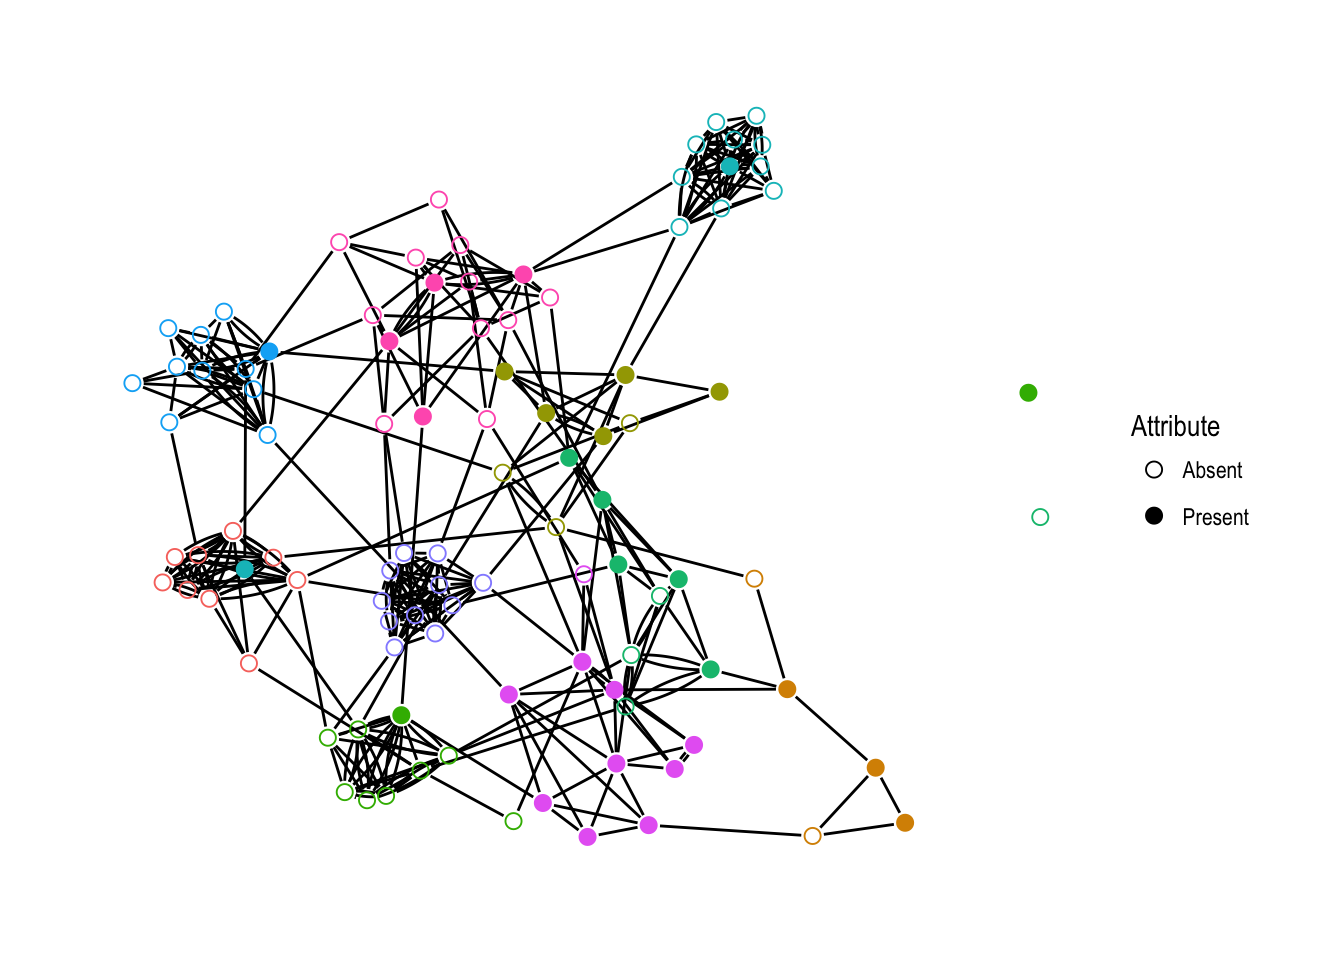
\includegraphics{thesis_files/figure-latex/example-net-1} 

}

\caption{A simulated network with 100 vertices, colored according to neighborhood. The vertex fill indicates the presence or absence of the simulated attribute.}\label{fig:example-net}
\end{figure}
\begin{figure}

{\centering 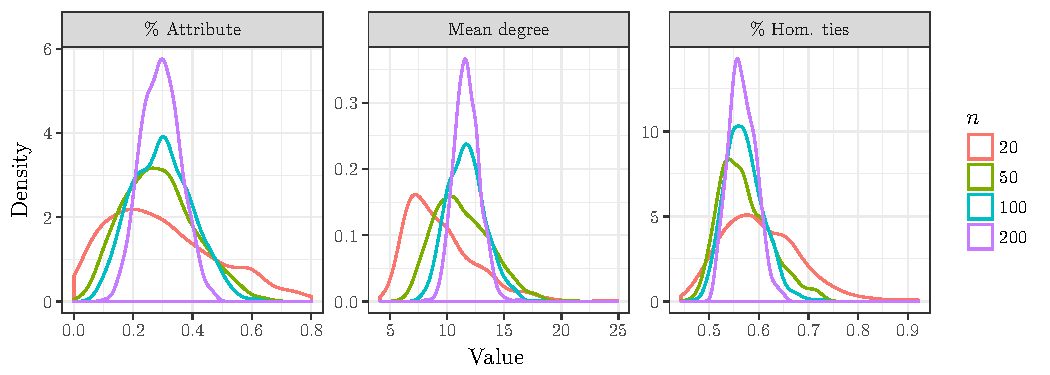
\includegraphics{thesis_files/figure-latex/asymp-dens-1} 

}

\caption{Density plots of simulated statistics of locally dependent random networks.}\label{fig:asymp-dens}
\end{figure}
\begin{figure}

{\centering 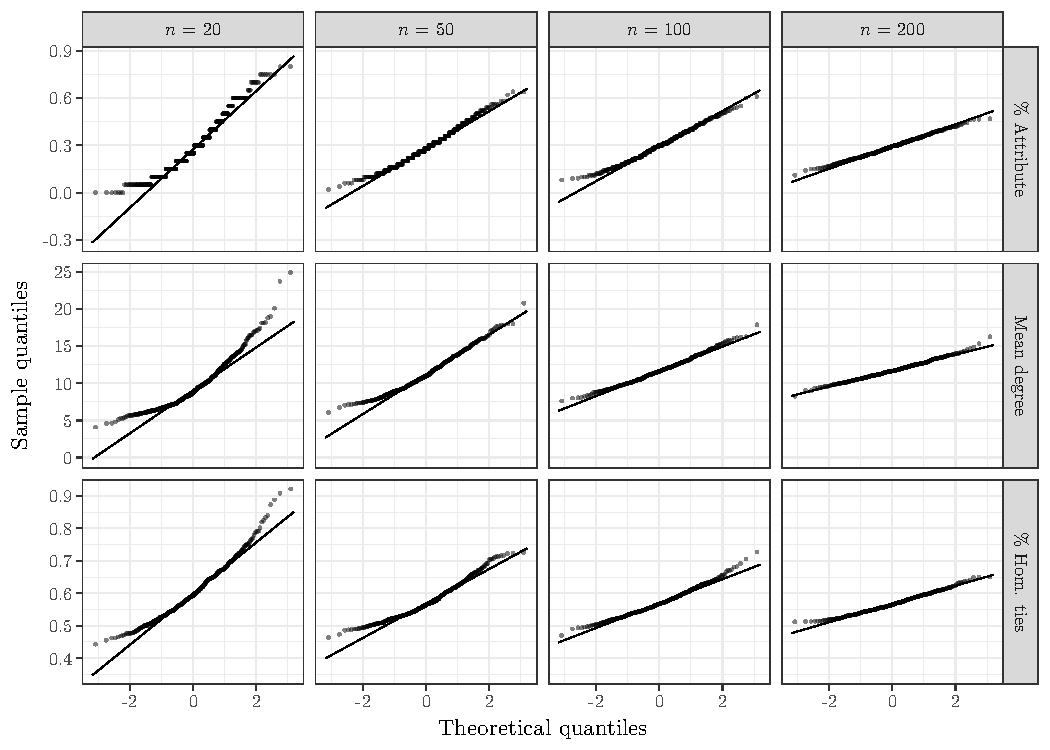
\includegraphics{thesis_files/figure-latex/asymp-qq-1} 

}

\caption{Normal Q-Q plots for simulated statistics of locally dependent random networks.}\label{fig:asymp-qq}
\end{figure}
\section{Standard error estimation}\label{standard-error-estimation}

Given the asymptotic normality, all that remains to make these theorems
useful for inference is to find a method to estimate the standard error
of a statistic from a single observation. To that end, here we simulate
a single network with 200 vertices by the same procedure as above and
attempt to recover the standard errors of the statistics. We can compare
these estimates to the standard errors of the empirical distributions we
found in our previous simulation.

There are several approaches to approximating the standard errors. The
first is to follow the vertex-level jackknife procedure outlined by
Snijders \& Borgatti (\protect\hyperlink{ref-Snijders1999}{1999}). This
method is a modification of the standard jackknife estimator of standard
deviation. At each iteration of the procedure, we remove one vertex from
the network and recalculate the statistics of interest. Then we estimate
the standard error with the equation
\begin{equation}
\widehat{\text{s.e.}} = \sqrt{\frac{n - 2}{2n} \sum_{i = 1}^{n} (g_{-i} - \bar{g})^2},
\end{equation}
where \(g\) is the quantity whose standard error we are approximating
and \(g_{-i}\) is \(g\) calculated with vertex \(i\) removed. This
differs from the standard jackknife estimator in the multiplicative
constant. Heuristically, this constant accounts for the fact that we are
seeing much less variation in the jackknife networks than we would
expect to see in the true distribution. This follows from the fact that
the variance of a statistic of the edge variables is (approximately)
inversely proportional to the number of edge variables, \(n(n-1)\), not
the number of vertices, \(n\) (Snijders \& Borgatti,
\protect\hyperlink{ref-Snijders1999}{1999}). We can see in Table
\ref{tab:se-jack} that this procedure underestimates the variance of our
statistics.
\begin{table}

\caption{\label{tab:se-jack}Standard error estimates using the jackknife at the vertex level.}
\centering
\begin{tabular}[t]{lrr}
\toprule
Statistic & Simulated standard error & Jackknife standard error\\
\midrule
\% Attribute & 0.0694576 & 0.0245443\\
Mean degree & 1.2062191 & 0.6020049\\
\% Hom. ties & 0.0262896 & 0.0204720\\
\bottomrule
\end{tabular}
\end{table}
\begin{table}

\caption{\label{tab:se-jack2}Standard error estimates using the jackknife at the neighborhood level.}
\centering
\begin{tabular}[t]{lrr}
\toprule
Statistic & Simulated standard error & Jackknife standard error\\
\midrule
\% Attribute & 0.0694576 & 0.0615096\\
Mean degree & 1.2062191 & 1.2017300\\
\% Hom. ties & 0.0262896 & 0.0316870\\
\bottomrule
\end{tabular}
\end{table}
This is most likely because of the dependence between vertices in the
process that generated the network.

The second method is a standard jackknife, but leverages the
neighborhood structure and the local dependence of the network. We do
this by applying the jackknife at the level of the neighborhoods. That
is to say, we remove each neighborhood in turn and recompute the
statistic and then compute the jackknife estimator
\begin{equation}
\widehat{\text{s.e.}} = \sqrt{\frac{m-1}{m} \sum_{i = 1}^m (g_{-i} - \bar{g})^2},
\end{equation}
where \(m\) is the number of neighborhoods. This process gives much more
appropriate estimates, shown in Table \ref{tab:se-jack2}.

\section{Discussion of future work}\label{discussion-of-future-work}

Further development of locally dependent ERNMs for modelling complex
social processes will have major impacts in the social sciences. The
most pressing issue is the creation of software that allows for
estimating parameters in these models. Code for fitting locally
dependent ERGMs was developed by Schweinberger \& Handcock
(\protect\hyperlink{ref-Schweinberger2015}{2015}) and a Markov chain
Monte Carlo algorithm for ERNMs was implemented by Fellows \& Handcock
(\protect\hyperlink{ref-Fellows2012}{2012}). However, it still remains
to combine these two developments to work with locally dependent ERNMs.

Further mathematical work is also required to extend Theorem
\ref{thm:norm3} to statistics involving more than one vertex attribute.
This proof requires a multivariate analogue of the central limit theorem
for \(M\)-dependent random variables. As my adviser told me, where there
is a univariate central limit theorem, there is invariably a
corresponding multidimensional theorem. However, we are unable to find a
proof of this, so that result must be the topic of future work.

Finally, an investigation into the properties of standard error
estimates like those produced above is much needed. Network sample sizes
tend to be relatively small, so being forced to aggregate at the
neighborhood level is a nontrivial issue. Furthermore, the jackknife
procedure is most likely not making full use of all the information
available within the observed network. However, a bootstrap procedure
is, as far as my research shows, undefined for network data. Difficulty
comes from being unable to sample with replacement. If one were to
sample a network's vertices or edges with replacement, most likely
duplicate edges would appear in the resampled networks. It is unclear
how duplicates should be handled when calculating network statistics, so
that sort of procedure is difficult to define.

\appendix


\chapter{Code}\label{code}

All source materials used to write this thesis are available in the Reed
College Library's digital thesis archive. This appendix contains the
most important code used in the final chapter.

\section{Network simulation code}\label{network-simulation-code}
\begin{Shaded}
\begin{Highlighting}[]
\NormalTok{if(!}\KeywordTok{require}\NormalTok{(devtools))}
  \KeywordTok{install.packages}\NormalTok{(}\StringTok{"devtools"}\NormalTok{, }\DataTypeTok{repos =} \StringTok{"http://cran.rstudio.com"}\NormalTok{)}
\NormalTok{if(!}\KeywordTok{require}\NormalTok{(thesisdown))}
  \NormalTok{devtools::}\KeywordTok{install_github}\NormalTok{(}\StringTok{"ismayc/thesisdown"}\NormalTok{)}
\KeywordTok{library}\NormalTok{(thesisdown)}

\KeywordTok{library}\NormalTok{(statnet)}
\KeywordTok{library}\NormalTok{(Bergm)}
\KeywordTok{library}\NormalTok{(tidyverse)}
\KeywordTok{library}\NormalTok{(broom)}
\KeywordTok{library}\NormalTok{(ggraph)}
\KeywordTok{library}\NormalTok{(purrr)}
\KeywordTok{library}\NormalTok{(Rcpp)}
\KeywordTok{library}\NormalTok{(knitr)}
\end{Highlighting}
\end{Shaded}
The following C++ code, compiled into a shared library using the
\texttt{Rcpp} package, gives function definitions used in simulating
networks (Eddelbuettel \& Francois,
\protect\hyperlink{ref-Eddelbuettel2011}{2011}).
\begin{Shaded}
\begin{Highlighting}[]
\OtherTok{#include <Rcpp.h>}

\KeywordTok{using} \KeywordTok{namespace} \NormalTok{Rcpp;}

\CommentTok{//[[Rcpp::export]]}
\NormalTok{IntegerMatrix make_adj(List vert_df)\{}
  \NormalTok{NumericVector vert = vert_df[}\StringTok{"vert"}\NormalTok{];}
  \NormalTok{NumericVector nbhd = vert_df[}\StringTok{"nbhd"}\NormalTok{];}
  \NormalTok{NumericVector grp = vert_df[}\StringTok{"grp"}\NormalTok{];}
  \DataTypeTok{double} \NormalTok{n = vert.size();}
  
  \NormalTok{IntegerMatrix adj_mat(n,n);}
  
  \KeywordTok{for}\NormalTok{(}\DataTypeTok{int} \NormalTok{i = }\DecValTok{0}\NormalTok{; i < n; i++)\{}
    \KeywordTok{for}\NormalTok{(}\DataTypeTok{int} \NormalTok{j = }\DecValTok{0}\NormalTok{; j < n; j++)\{}
      \KeywordTok{if}\NormalTok{(nbhd[i] == nbhd[j])\{}
        \KeywordTok{if}\NormalTok{(grp[i] == grp[j])\{}
          \NormalTok{adj_mat(i,j) = as<}\DataTypeTok{int}\NormalTok{>(rbinom(}\DecValTok{1}\NormalTok{,}\DecValTok{1}\NormalTok{,}\FloatTok{.3}\NormalTok{));}
          \KeywordTok{continue}\NormalTok{;}
        \NormalTok{\} }\KeywordTok{else} \NormalTok{\{}
          \NormalTok{adj_mat(i,j) = as<}\DataTypeTok{int}\NormalTok{>(rbinom(}\DecValTok{1}\NormalTok{, }\DecValTok{1}\NormalTok{, }\FloatTok{.1}\NormalTok{));}
          \KeywordTok{continue}\NormalTok{;}
          \NormalTok{\}}
      \NormalTok{\} }\KeywordTok{else}\NormalTok{\{       }
        \NormalTok{adj_mat(i,j) = as<}\DataTypeTok{int}\NormalTok{>(rbinom(}\DecValTok{1}\NormalTok{, }\DecValTok{1}\NormalTok{, }\DecValTok{50}\NormalTok{/(n*n)));}
        \KeywordTok{continue}\NormalTok{;}
      \NormalTok{\}}
    \NormalTok{\}}
  \NormalTok{\}}

  \KeywordTok{for}\NormalTok{(}\DataTypeTok{int} \NormalTok{i = }\DecValTok{1}\NormalTok{; i < n/}\DecValTok{10}\NormalTok{; i++)\{}
    \KeywordTok{for}\NormalTok{(}\DataTypeTok{int} \NormalTok{j = }\DecValTok{0}\NormalTok{; j < n; j++)\{}
      \KeywordTok{for}\NormalTok{(}\DataTypeTok{int} \NormalTok{k = }\DecValTok{0}\NormalTok{; k < n; k++)\{}
        \KeywordTok{for}\NormalTok{(}\DataTypeTok{int} \NormalTok{l = }\DecValTok{0}\NormalTok{; l < n; l++)\{}
          \KeywordTok{if}\NormalTok{(nbhd[j] == i &&}
             \NormalTok{nbhd[k] == i &&}
             \NormalTok{nbhd[l] == i)\{}
            \KeywordTok{if}\NormalTok{(adj_mat(j, k) == }\DecValTok{1} \NormalTok{&&}
               \NormalTok{adj_mat(k, l) == }\DecValTok{1} \NormalTok{&&}
               \NormalTok{adj_mat(j, l) == }\DecValTok{0}\NormalTok{)\{}
              \NormalTok{adj_mat(j, l) = as<}\DataTypeTok{int}\NormalTok{>(rbinom(}\DecValTok{1}\NormalTok{, }\DecValTok{1}\NormalTok{, }\FloatTok{.75}\NormalTok{));}
            \NormalTok{\}}
          \NormalTok{\}}
        \NormalTok{\}}
      \NormalTok{\}}
    \NormalTok{\}}
  \NormalTok{\}}

  \KeywordTok{return} \NormalTok{adj_mat;}
\NormalTok{\}}

\CommentTok{//[[Rcpp::export]]}
\NormalTok{IntegerVector make_attr(List vert_df, IntegerMatrix adj_mat)\{}
  \NormalTok{IntegerVector attr = vert_df[}\StringTok{"attr"}\NormalTok{];}
  \NormalTok{IntegerVector nbhd = vert_df[}\StringTok{"nbhd"}\NormalTok{];}
  \DataTypeTok{int} \NormalTok{n = attr.size();}
  \KeywordTok{for}\NormalTok{(}\DataTypeTok{int} \NormalTok{i = }\DecValTok{0}\NormalTok{; i < n; i++)\{}
    \KeywordTok{for}\NormalTok{(}\DataTypeTok{int} \NormalTok{j = }\DecValTok{0}\NormalTok{; j < n; j++)\{}
      \KeywordTok{if}\NormalTok{(attr[i] == }\DecValTok{1} \NormalTok{&& adj_mat(i,j) == }\DecValTok{1} \NormalTok{&& nbhd[i] == nbhd[j])\{}
        \NormalTok{attr[j] = as<}\DataTypeTok{int}\NormalTok{>(rbinom(}\DecValTok{1}\NormalTok{, }\DecValTok{1}\NormalTok{, }\FloatTok{.75}\NormalTok{));}
      \NormalTok{\}}\KeywordTok{else} \KeywordTok{if}\NormalTok{(adj_mat(i,j) == }\DecValTok{1} \NormalTok{&& nbhd[i] == nbhd[j])\{}
        \NormalTok{attr[j] = as<}\DataTypeTok{int}\NormalTok{>(rbinom(}\DecValTok{1}\NormalTok{, }\DecValTok{1}\NormalTok{, }\FloatTok{.1}\NormalTok{));}
      \NormalTok{\}}
    \NormalTok{\}}
  \NormalTok{\}}
  \KeywordTok{return} \NormalTok{attr;}
\NormalTok{\}}
\end{Highlighting}
\end{Shaded}
This R code generates networks and computes the three chosen statistics
for each one. The final result is a data set of networks and
corresponding statistics used to produce density and quantile-quantile
plots.
\begin{Shaded}
\begin{Highlighting}[]
\NormalTok{make_net <-}\StringTok{ }\NormalTok{function(n)\{}
  \NormalTok{vert_df <-}\StringTok{ }\KeywordTok{tibble}\NormalTok{(}\DataTypeTok{vert =} \DecValTok{1}\NormalTok{:n)}
  \NormalTok{nbhds <-}\StringTok{ }\DecValTok{1}\NormalTok{:}\KeywordTok{floor}\NormalTok{(n/}\DecValTok{10}\NormalTok{)}
  \NormalTok{vert_df <-}\StringTok{ }\NormalTok{vert_df %>%}\StringTok{ }
\StringTok{    }\KeywordTok{mutate}\NormalTok{(}\DataTypeTok{nbhd =} \KeywordTok{sample}\NormalTok{(nbhds, n, }\DataTypeTok{replace =} \OtherTok{TRUE}\NormalTok{),}
           \DataTypeTok{grp =} \KeywordTok{rbinom}\NormalTok{(n, }\DecValTok{1}\NormalTok{, .}\DecValTok{5}\NormalTok{),}
           \DataTypeTok{attr =} \KeywordTok{rbinom}\NormalTok{(n, }\DecValTok{1}\NormalTok{, .}\DecValTok{3}\NormalTok{))}
  
  \NormalTok{adj_mat <-}\StringTok{ }\KeywordTok{make_adj}\NormalTok{(vert_df)}
  
  \NormalTok{vert_df$attr <-}\StringTok{ }\KeywordTok{make_attr}\NormalTok{(vert_df, adj_mat)}
  
  \NormalTok{net <-}\StringTok{ }\KeywordTok{network}\NormalTok{(adj_mat)}
  \NormalTok{net %v%}\StringTok{ "group"} \NormalTok{<-}\StringTok{ }\NormalTok{vert_df$grp}
  \NormalTok{net %v%}\StringTok{ "attribute"} \NormalTok{<-}\StringTok{ }\NormalTok{vert_df$attr}
  \NormalTok{net %v%}\StringTok{ "nbhd"} \NormalTok{<-}\StringTok{ }\NormalTok{vert_df$nbhd}
  
  \KeywordTok{return}\NormalTok{(net)}
\NormalTok{\}}

\NormalTok{node_match <-}\StringTok{ }\NormalTok{function(net)\{}
  \NormalTok{edge_list <-}\StringTok{ }\KeywordTok{as.edgelist}\NormalTok{(net)}
  \NormalTok{grps <-}\StringTok{ }\NormalTok{net %v%}\StringTok{ "group"}
  \NormalTok{num <-}\StringTok{ }\DecValTok{0}
  \NormalTok{for(i in }\DecValTok{1}\NormalTok{:}\KeywordTok{nrow}\NormalTok{(edge_list))\{}
    \NormalTok{if(grps[edge_list[i, }\DecValTok{1}\NormalTok{]] ==}\StringTok{ }\NormalTok{grps[edge_list[i,}\DecValTok{2}\NormalTok{]]) num <-}\StringTok{ }\NormalTok{num +}\StringTok{ }\DecValTok{1}
  \NormalTok{\}}
  \NormalTok{num/}\KeywordTok{nrow}\NormalTok{(edge_list)}
\NormalTok{\}}
\NormalTok{n_reps <-}\StringTok{ }\DecValTok{500}
\NormalTok{results <-}\StringTok{ }\KeywordTok{tibble}\NormalTok{(}\DataTypeTok{num =} \KeywordTok{c}\NormalTok{(}\KeywordTok{rep}\NormalTok{(}\DecValTok{20}\NormalTok{, n_reps),}
                        \KeywordTok{rep}\NormalTok{(}\DecValTok{50}\NormalTok{, n_reps),}
                        \KeywordTok{rep}\NormalTok{(}\DecValTok{100}\NormalTok{, n_reps),}
                        \KeywordTok{rep}\NormalTok{(}\DecValTok{200}\NormalTok{, n_reps)))}
\NormalTok{results <-}\StringTok{ }\NormalTok{results %>%}\StringTok{ }
\StringTok{  }\KeywordTok{mutate}\NormalTok{(}\DataTypeTok{net =} \KeywordTok{map}\NormalTok{(num, make_net),}
         \DataTypeTok{mean_deg =} \KeywordTok{map_dbl}\NormalTok{(net, ~}\StringTok{ }\KeywordTok{mean}\NormalTok{(}\KeywordTok{degree}\NormalTok{(.x))),}
         \DataTypeTok{mean_attr =} \KeywordTok{map_dbl}\NormalTok{(net, ~}\StringTok{ }\KeywordTok{mean}\NormalTok{(.x %v%}\StringTok{ "attribute"}\NormalTok{)),}
         \DataTypeTok{prop_homo =} \KeywordTok{map_dbl}\NormalTok{(net, node_match))}

\NormalTok{results <-}\StringTok{ }\NormalTok{results %>%}\StringTok{ }
\StringTok{  }\KeywordTok{gather}\NormalTok{(stat, value, -(num:net))}
\end{Highlighting}
\end{Shaded}
\section{Jackknife standard error
code}\label{jackknife-standard-error-code}

This code computes the neighborhood level standard error estimates for
statistics of the graph.
\begin{Shaded}
\begin{Highlighting}[]
\NormalTok{n_vert <-}\StringTok{ }\DecValTok{200}
\NormalTok{net <-}\StringTok{ }\KeywordTok{make_net}\NormalTok{(n_vert)}

\NormalTok{nbhds <-}\StringTok{ }\NormalTok{net %v%}\StringTok{ "nbhd"}
\NormalTok{num_nbhds <-}\StringTok{ }\KeywordTok{length}\NormalTok{(}\KeywordTok{unique}\NormalTok{(nbhds))}
\NormalTok{boot3 <-}\StringTok{ }\KeywordTok{numeric}\NormalTok{(num_nbhds)}

\NormalTok{jack_df <-}\StringTok{ }\KeywordTok{tibble}\NormalTok{(}\DataTypeTok{mean_deg =} \KeywordTok{numeric}\NormalTok{(num_nbhds),}
                  \DataTypeTok{mean_attr =} \KeywordTok{numeric}\NormalTok{(num_nbhds),}
                  \DataTypeTok{prop_homo =} \KeywordTok{numeric}\NormalTok{(num_nbhds))}

\NormalTok{for(i in }\DecValTok{1}\NormalTok{:num_nbhds)\{}
  \NormalTok{temp_net <-}\StringTok{ }\KeywordTok{rm_vertex}\NormalTok{(net, }\KeywordTok{which}\NormalTok{(nbhds ==}\StringTok{ }\NormalTok{i))}
  \NormalTok{jack_df$mean_deg[i] <-}\StringTok{ }\KeywordTok{mean}\NormalTok{(}\KeywordTok{degree}\NormalTok{(temp_net))}
  \NormalTok{jack_df$mean_attr[i] <-}\StringTok{ }\KeywordTok{mean}\NormalTok{(temp_net %v%}\StringTok{ "attribute"}\NormalTok{)}
  \NormalTok{jack_df$prop_homo[i] <-}\StringTok{ }\KeywordTok{node_match}\NormalTok{(temp_net)}
\NormalTok{\}}

\NormalTok{jack_df <-}\StringTok{ }\NormalTok{jack_df %>%}\StringTok{ }
\StringTok{  }\KeywordTok{gather}\NormalTok{(stat, value) %>%}\StringTok{ }
\StringTok{  }\KeywordTok{group_by}\NormalTok{(stat) %>%}\StringTok{ }
\StringTok{  }\KeywordTok{summarise}\NormalTok{(}\DataTypeTok{jack_sd =} \KeywordTok{sqrt}\NormalTok{((num_nbhds -}\StringTok{ }\DecValTok{1}\NormalTok{)/num_nbhds *}\StringTok{ }
\StringTok{                             }\KeywordTok{sum}\NormalTok{((value -}\StringTok{ }\KeywordTok{mean}\NormalTok{(value))^}\DecValTok{2}\NormalTok{)))}
\end{Highlighting}
\end{Shaded}
\backmatter

\chapter*{References}\label{references}
\addcontentsline{toc}{chapter}{References}

\markboth{References}{References}

\noindent

\setlength{\parindent}{-0.20in} \setlength{\leftskip}{0.20in}
\setlength{\parskip}{8pt}

\hypertarget{refs}{}
\hypertarget{ref-Billingsley1995}{}
Billingsley, P. (1995). \emph{Probability and measure} (3. ed.,
authorized reprint). New Delhi: Wiley India.

\hypertarget{ref-Caimo2011}{}
Caimo, A., \& Friel, N. (2011). Bayesian inference for exponential
random graph models. \emph{Social Networks}, \emph{33}(1), 41--55.
\url{http://doi.org/10.1016/j.socnet.2010.09.004}

\hypertarget{ref-Caimo2014}{}
Caimo, A., \& Friel, N. (2014). Bergm: Bayesian exponential random
graphs in R. \emph{Journal of Statistical Software}, \emph{61}(2).
Retrieved from \url{http://www.jstatsoft.org/v61/i02/}

\hypertarget{ref-Eddelbuettel2013}{}
Eddelbuettel, D. (2013). \emph{Seamless R and C++ integration with
rcpp}. New York: Springer.

\hypertarget{ref-Eddelbuettel2011}{}
Eddelbuettel, D., \& Francois, R. (2011). Rcpp: Seamless R and C++
integration. \emph{Journal of Statistical Software}, (40, 8).

\hypertarget{ref-Fellows2012}{}
Fellows, I., \& Handcock, M. S. (2012). Exponential-family random
network models. \emph{ArXiv Preprint ArXiv:1208.0121}.

\hypertarget{ref-Geyer1992}{}
Geyer, Charles J., \& Thompson, E. A. (1992). Constrained monte carlo
maximum likelihood for dependent data. \emph{Journal of the Royal
Statistical Society. Series B (Methodological)}, \emph{54}(3), 657--699.
Retrieved from \url{http://www.jstor.org/stable/2345852}

\hypertarget{ref-Groendyke2012}{}
Groendyke, C., Welch, D., \& Hunter, D. R. (2012). A network-based
analysis of the 1861~Hagelloch measles data. \emph{Biometrics},
\emph{68}(3), 755--765.
\url{http://doi.org/10.1111/j.1541-0420.2012.01748.x}

\hypertarget{ref-Handcock2016a}{}
Handcock, M. S., Hunter, D. R., Butts, C. T., Goodreau, S. M.,
Krivitsky, P. N., \& Morris, M. (2016). \emph{ergm: Fit, simulate and
diagnose exponential-family models for networks}. The Statnet Project
(\url{http://www.statnet.org}). Retrieved from
\url{http://CRAN.R-project.org/package=ergm}

\hypertarget{ref-Hunter2008}{}
Hunter, D. R., Handcock, M. S., Butts, C. T., Goodreau, S. M., \&
Morris, M. (2008). ergm: A package to fit, simulate and diagnose
exponential-family models for networks. \emph{Journal of Statistical
Software}, \emph{24}(3).

\hypertarget{ref-Ismay}{}
Ismay, C. (2017). \emph{thesisdown: An updated R Markdown thesis
template using the bookdown package}.

\hypertarget{ref-Morris2008}{}
Morris, M., Handcock, M. S., \& Hunter, D. R. (2008). Specification of
exponential-family random graph models: Terms and computational aspects.
\emph{Journal of Statistical Software}, \emph{24}(4).

\hypertarget{ref-Murray2012}{}
Murray, I., Ghahramani, Z., \& MacKay, D. (2012). MCMC for
doubly-intractable distributions. \emph{ArXiv Preprint ArXiv:1206.6848}.

\hypertarget{ref-Robinson2016}{}
Robinson, D. (2016). \emph{Broom: Convert statistical analysis objects
into tidy data frames}. Retrieved from
\url{https://CRAN.R-project.org/package=broom}

\hypertarget{ref-Schweinberger2015}{}
Schweinberger, M., \& Handcock, M. S. (2015). Local dependence in random
graph models: Characterization, properties and statistical inference.
\emph{Journal of the Royal Statistical Society: Series B (Statistical
Methodology)}, \emph{77}(3), 647--676.

\hypertarget{ref-Shalizi2013}{}
Shalizi, C. R., \& Rinaldo, A. (2013). Consistency under sampling of
exponential random graph models. \emph{The Annals of Statistics},
\emph{41}(2), 508--535. \url{http://doi.org/10.1214/12-AOS1044}

\hypertarget{ref-Snijders1999}{}
Snijders, T. A. B., \& Borgatti, S. P. (1999). Non-parametric standard
errors and tests for network statistics. \emph{Connections},
\emph{22}(2), 61--70.

\hypertarget{ref-Strauss1990}{}
Strauss, D., \& Ikeda, M. (1990). Pseudolikelihood estimation for social
networks. \emph{Journal of the American Statistical Association},
\emph{85}(409), 204--212. Retrieved from
\url{http://www.jstor.org/stable/2289546}

\hypertarget{ref-Wasserman2004}{}
Wasserman, L. (2004). \emph{All of statistics}. New York:
Springer-Verlag.

\hypertarget{ref-Wasserman1996}{}
Wasserman, S., \& Pattison, P. (1996). Logit models and logistic
regressions for social networks: I. an introduction to markov graphs and
p*. \emph{Psychometrika}, \emph{61}(3), 401--425.

\hypertarget{ref-Wickham2016a}{}
Wickham, H. (2016a). \emph{Purrr: Functional programming tools}.
Retrieved from \url{https://CRAN.R-project.org/package=purrr}

\hypertarget{ref-Wickham2016}{}
Wickham, H. (2016b). \emph{Tidyverse: Easily install and load
'tidyverse' packages}. Retrieved from
\url{https://CRAN.R-project.org/package=tidyverse}

\hypertarget{ref-Xie2016}{}
Xie, Y. (2016). knitr: A general-purpose package for dynamic report
generation in R (Version R package version 1.15.19).


% Index?

\end{document}
